\documentclass[12pt,a4paper]{report}

% =========================================================
% BIG DATA SYSTEMS (24CI51) - PROJECT / SELF-LEARNING REPORT
% DEPARTMENT OF CSE (ARTIFICIAL INTELLIGENCE & MACHINE LEARNING)
% M. S. RAMAIAH INSTITUTE OF TECHNOLOGY, BENGALURU
% =========================================================

% ---------------- Packages ----------------
\usepackage[a4paper,top=1.55in,bottom=1in,left=1.25in,right=1in,
            headheight=75pt,headsep=18pt]{geometry}
\usepackage{setspace}
\usepackage{times}
\usepackage{graphicx}
\usepackage{float}
\usepackage{array}
\usepackage{tabularx}
\usepackage{longtable}
\usepackage{titlesec}
\usepackage{tocloft}
\usepackage{fancyhdr}
\usepackage{hyperref}
\usepackage{ragged2e}
\usepackage{enumitem}
\usepackage{caption}
\usepackage{booktabs}
\usepackage{multirow}
\usepackage{xcolor}
\usepackage{listings}
\usepackage{amsmath,amssymb}

\hypersetup{
    colorlinks=true,
    linkcolor=black,
    urlcolor=blue!70!black,
    citecolor=black
}

\onehalfspacing
\setlength{\parindent}{0.5in}
\setlength{\parskip}{0pt}
\justifying
\setlist[itemize]{leftmargin=*}
\setlist[enumerate]{leftmargin=*}
\renewcommand{\arraystretch}{1.2}

% Code Listing Configuration
\definecolor{codegreen}{rgb}{0,0.6,0}
\definecolor{codegray}{rgb}{0.5,0.5,0.5}
\definecolor{codepurple}{rgb}{0.58,0,0.82}
\definecolor{backcolour}{rgb}{0.97,0.97,0.97}

\lstdefinestyle{mystyle}{
    backgroundcolor=\color{backcolour},   
    commentstyle=\color{codegreen},
    keywordstyle=\color{blue}\bfseries,
    numberstyle=\tiny\color{codegray},
    stringstyle=\color{codepurple},
    basicstyle=\ttfamily\footnotesize,
    breakatwhitespace=false,         
    breaklines=true,                 
    captionpos=b,                    
    keepspaces=true,                 
    numbers=left,                    
    numbersep=5pt,                  
    showspaces=false,                
    showstringspaces=false,
    showtabs=false,                  
    tabsize=2,
    frame=single
}
\lstset{style=mystyle}

% ---------------- Project Details ----------------
\newcommand{\ProjectTitle}{BIG DATA SYSTEMS: TECHNOLOGY STUDY AND IMPLEMENTATION}
\newcommand{\CourseCode}{24CI51 -- BIG DATA SYSTEMS}
\newcommand{\AcademicYear}{2025--2026}
\newcommand{\Department}{DEPARTMENT OF CSE (ARTIFICIAL INTELLIGENCE \& MACHINE LEARNING)}
\newcommand{\StudentOne}{Aditya Mundra}
\newcommand{\USNOne}{1MS22AI005}
\newcommand{\GuideOne}{Mr. Subash N}
\newcommand{\GuideDesignation}{Assistant Professor}
\newcommand{\HOD}{Dr. Siddesh G M}
\newcommand{\HODDesignation}{Professor \& Head}

% ---------------- Header/Footer ----------------
\newcommand{\RamaiahHeaderImage}{%
  
\includegraphics[width=1\textwidth,height=4cm,keepaspectratio]{images/rit_header.png}%
}

\pagestyle{fancy}
\fancyhf{}
\fancyhead[C]{\RamaiahHeaderImage}
\fancyfoot[L]{\small \AcademicYear}
\fancyfoot[C]{\small Big Data Systems (24CI51)}
\fancyfoot[R]{\small \thepage}
\renewcommand{\headrulewidth}{0pt}
\renewcommand{\footrulewidth}{0.4pt}

\fancypagestyle{plain}{%
  \fancyhf{}
  \fancyhead[C]{\RamaiahHeaderImage}
  \fancyfoot[L]{\small \AcademicYear}
  \fancyfoot[C]{\small Big Data Systems (24CI51)}
  \fancyfoot[R]{\small \thepage}
  \renewcommand{\headrulewidth}{0pt}
  \renewcommand{\footrulewidth}{0.4pt}
}

\titleformat{\chapter}[display]
  {\normalfont\bfseries\centering\Large}
  {\chaptername\ \thechapter}{10pt}{\Large}
\titleformat{\section}{\normalfont\bfseries\large}{\thesection}{1em}{}
\titleformat{\subsection}{\normalfont\bfseries}{\thesubsection}{1em}{}

\newcommand{\activityheading}[2]{%
  \section{Activity #1: #2}%
}
\newcommand{\insertfigure}[3][0.85\textwidth]{%
\begin{figure}[H]
    \centering
    \includegraphics[width=#1]{#2}
    \caption{#3}
    \label{fig:#2}
\end{figure}
}

\begin{document}

% =========================================================
% TITLE PAGE
% =========================================================
\begin{titlepage}
\centering
\thispagestyle{empty}

\vspace*{0.2cm}
{\bfseries\Large A REPORT ON\\[0.3cm]}
{\bfseries\LARGE \ProjectTitle\\[0.5cm]}

{\bfseries for the course\\[0.2cm]}
{\bfseries \CourseCode\\[0.6cm]}

Submitted in partial fulfillment of the academic requirements
for the course work of\\[0.2cm]
{\bfseries Bachelor of Engineering\\}
in\\
{\bfseries Computer Science and Engineering\\[0.2cm]}
{\bfseries (Artificial Intelligence \& Machine Learning)\\[0.6cm]}

{\bfseries Submitted by:\\[0.2cm]}
{\large \textbf{\StudentOne}\ (\textbf{\USNOne})\\[0.8cm]}

{\bfseries Under the Guidance of:\\[0.2cm]}
{\large \textbf{\GuideOne}\\[0.1cm]}
\GuideDesignation\\[0.8cm]

{\bfseries M. S. RAMAIAH INSTITUTE OF TECHNOLOGY\\}
\textit{(Autonomous Institute Affiliated to VTU, Approved by AICTE, Accredited by NAAC with `A+' Grade)}\\
{\bfseries BENGALURU -- 560054\\}
{\bfseries \AcademicYear}

\end{titlepage}

\pagenumbering{roman}
\setcounter{page}{1}

% =========================================================
% CERTIFICATE
% =========================================================
\chapter*{CERTIFICATE}
\addcontentsline{toc}{chapter}{Certificate}

Certified that the self-learning report entitled ``\ProjectTitle'' submitted by \textbf{\StudentOne} (USN: \textbf{\USNOne}), bonafide student of M. S. Ramaiah Institute of Technology, Bengaluru, is a record of the work carried out by him for the course \textbf{\CourseCode} during the academic year \textbf{\AcademicYear}. The report is submitted in partial fulfillment of the academic requirements prescribed by the institute for the award of Bachelor of Engineering in Computer Science and Engineering (Artificial Intelligence \& Machine Learning).

\vspace{2.5cm}

\begin{tabularx}{\textwidth}{X X}
\centering \textbf{Signature of the Guide} &
\centering\arraybackslash \textbf{Signature of the HoD}\\[0.5cm]
\centering \GuideOne &
\centering\arraybackslash \HOD\\
\centering \GuideDesignation &
\centering\arraybackslash \HODDesignation\\
\centering Department of CSE (AI \& ML) &
\centering\arraybackslash Department of CSE (AI \& ML)\\
\centering MSRIT, Bengaluru &
\centering\arraybackslash MSRIT, Bengaluru\\
\end{tabularx}

\clearpage

% =========================================================
% DECLARATION
% =========================================================
\chapter*{DECLARATION}
\addcontentsline{toc}{chapter}{Declaration}

I hereby declare that the report entitled ``\ProjectTitle'' is the authentic record of work carried out by me at M. S. Ramaiah Institute of Technology, Bengaluru, as part of the self-learning component for the course \textbf{\CourseCode}. The work presented in this report represents genuine study, simulation, and empirical software execution conducted by me and has not been submitted in part or full for the award of any other degree, diploma, or certificate.

\vspace{2.5cm}

\begin{flushright}
\begin{tabular}{l}
\textbf{Signature:}\\[1.0cm]
\textbf{\StudentOne}\\
USN: \textbf{\USNOne}\\
Department of CSE (AI \& ML)\\
M. S. Ramaiah Institute of Technology\\
Bengaluru -- 560054
\end{tabular}
\end{flushright}

\clearpage

% =========================================================
% ACKNOWLEDGEMENT
% =========================================================
\chapter*{ACKNOWLEDGEMENT}
\addcontentsline{toc}{chapter}{Acknowledgement}

I express my heartfelt gratitude to the management and Principal of \textbf{M. S. Ramaiah Institute of Technology} for providing the academic infrastructure, laboratories, and computational facilities necessary to carry out this self-learning activity.

I extend my sincere gratitude to \textbf{\HOD}, Professor \& Head, Department of CSE (Artificial Intelligence \& Machine Learning), for his continuous encouragement, academic support, and administrative guidance throughout the course.

I express my deepest gratitude to my course guide and faculty instructor, \textbf{\GuideOne}, \GuideDesignation, Department of CSE (AI \& ML), for his invaluable advice, technical reviews, constructive feedback, and patient guidance throughout the design and execution of these five Big Data activities.

I would also like to thank the technical staff of the department and my peers for their valuable discussions, collaborative insights, and support during the course of this study.

\vspace{1.5cm}
\begin{flushright}
\textbf{\StudentOne}\\
USN: \textbf{\USNOne}
\end{flushright}

\clearpage

% =========================================================
% ABSTRACT
% =========================================================
\chapter*{ABSTRACT}
\addcontentsline{toc}{chapter}{Abstract}

Modern enterprise computing environments generate vast, continuous, and structurally heterogeneous data volumes characterized by high velocity, volume, and variety. Traditional relational database management systems (RDBMS) fail to scale horizontally when processing distributed historical transactions, continuous telemetry streams, and polymorphic documents. This report presents an extensive study and prototype implementation across five foundational Big Data technologies: \textbf{Apache Hive}, \textbf{Apache Kafka}, \textbf{Apache Flink}, \textbf{MongoDB}, and \textbf{Cloud-Based Serverless Big Data Analytics (Amazon Web Services S3 and Athena)}.

In \textbf{Activity 1}, a multi-dimensional retail sales data warehouse was implemented using Apache Hive over 35,543 transactions across five supermarket branches. Leveraging vectorized Tez DAG execution and partitioned, bucketed Optimized Row Columnar (ORC) storage, HiveQL queries revealed bimodal shopping peaks (11:00 AM--1:00 PM and 5:00 PM--8:00 PM) and demonstrated that high-margin staple items generate 22\% of total revenue despite lower raw unit volumes. In \textbf{Activity 2}, a distributed Apache Kafka messaging cluster was constructed to ingest IoT traffic sensor telemetry across major smart city junctions. Using Murmur2 partition key hashing and multi-threaded consumer processing, the system evaluated speed and volume thresholds, emitting automated critical congestion alerts within 40 milliseconds. In \textbf{Activity 3}, Apache Flink was employed to monitor streaming biometric patient telemetry. Combining immediate threshold alerts with 20-second Tumbling Event-Time Windows, Flink reliably isolated sustained clinical episodes (tachycardia and hypoxemia) while filtering out transient sensor disconnect noise. In \textbf{Activity 4}, MongoDB demonstrated dynamic document storage for an e-commerce catalog; empirical query benchmarking via \texttt{explain()} proved that a compound B-Tree index reduced disk document scans by 90.3\% compared to full collection scans. Finally, in \textbf{Activity 5}, a serverless cloud log analytics lake was architected using AWS S3, AWS Glue, and Amazon Athena, isolating an application payment gateway outage and demonstrating a 95.4\% cost reduction over dedicated EC2 clusters. All activities were empirically verified on an interactive local PC execution harness, establishing an end-to-end perspective on contemporary Big Data engineering.

\clearpage

\tableofcontents
\clearpage
\listoffigures
\addcontentsline{toc}{chapter}{List of Figures}
\clearpage
\listoftables
\addcontentsline{toc}{chapter}{List of Tables}
\clearpage

\pagenumbering{arabic}

% =========================================================
% CHAPTER 1 - INTRODUCTION
% =========================================================
\chapter{INTRODUCTION}

\section{Introduction to Big Data Systems}
In the contemporary digital era, computing systems generate exponential data volumes originating from diverse sources such as mobile devices, point-of-sale terminals, Internet of Things (IoT) sensors, health monitors, and cloud microservice logs. This paradigm, commonly termed \textbf{Big Data}, is formally characterized by the \textbf{5 Vs}:
\begin{enumerate}
    \item \textbf{Volume:} Gigabytes to petabytes of structured and unstructured information requiring distributed file systems such as the Hadoop Distributed File System (HDFS) and cloud object stores (Amazon S3).
    \item \textbf{Velocity:} High-speed data generation demanding real-time ingestion backbones (Apache Kafka) and low-latency continuous stream-processing engines (Apache Flink).
    \item \textbf{Variety:} Multi-modal data formats spanning tabular relational rows, JSON documents, semi-structured server logs, and binary sensor packets.
    \item \textbf{Veracity:} Data noise, out-of-order event arrivals, and incomplete sensor readings requiring stateful windowed validation.
    \item \textbf{Value:} Extracting operational intelligence, customer insights, anomaly detection, and automated decisions through scalable analytics.
\end{enumerate}

Traditional monolithic relational database management systems (RDBMS) rely on scale-up (vertical) architectures with rigid schemas and heavy ACID locking mechanisms. Consequently, they fail when subjected to distributed batch aggregation over historical records or high-frequency streaming writes. Modern Big Data systems solve these bottlenecks by decoupling compute from storage, partitioning datasets across distributed worker clusters, and adopting specialized computational models: batch data warehousing (Apache Hive), distributed pub/sub messaging (Apache Kafka), event-time stream processing (Apache Flink), dynamic document storage (MongoDB), and serverless cloud data lakes (AWS Athena).

\section{Problem Definition}
This self-learning course work addresses five realistic industry scenarios spanning distinct data-processing archetypes:
\begin{enumerate}
    \item \textbf{Retail Sales Analytics (Batch Warehousing):} A hypermarket chain generates millions of daily POS transaction records. Management lacks visibility into branch-wise market shares, peak footfall hours, and product margins to guide inventory replenishment.
    \item \textbf{Smart City Traffic Control (Message Ingestion):} Traffic management centers receive continuous speed and vehicle-count telemetry from junction sensors. Delayed event ingestion prevents timely signal timing adjustments and route diversion broadcasts.
    \item \textbf{Clinical Patient Monitoring (Stream Processing):} Hospital ICUs track continuous biometric vitals (Heart Rate, $\text{SpO}_2$, Temperature). Clinicians suffer from alarm fatigue caused by transient sensor spikes and require windowed trend summaries for clinical review.
    \item \textbf{E-Commerce Product Catalog (NoSQL Document Store):} An online retailer manages polymorphic items across electronics, fashion, and books. Schema alterations in relational databases cause locking and downtime, requiring a dynamic schema database with high-performance indexing.
    \item \textbf{Cloud Application Log Lake (Serverless Analytics):} An online service provider generates gigabytes of access logs daily. The operations team needs to detect error spikes and latency degradation without provisioning expensive dedicated cluster infrastructure.
\end{enumerate}

\section{Objectives}
The primary objectives of this self-learning work are:
\begin{itemize}
    \item Study the architectural paradigms, metastore mechanics, and vectorized query execution of \textbf{Apache Hive}.
    \item Design and implement a partitioned, bucketed ORC data warehouse to analyze retail transaction velocity and derive inventory planning strategies.
    \item Understand the distributed commit log architecture, partition allocation, and consumer group offset management in \textbf{Apache Kafka}.
    \item Simulate real-time IoT sensor telemetry in Kafka and evaluate dual-threshold congestion rules to fire automated operator alerts.
    \item Investigate \textbf{Apache Flink}'s stateful stream processing, event-time semantics, watermarks, and tumbling windows.
    \item Build a Flink streaming pipeline to detect acute biometric emergencies while suppressing transient sensor noise through 20-second window aggregations.
    \item Analyze the document-oriented data model of \textbf{MongoDB} and empirically benchmark compound B-Tree index scans (\texttt{IXSCAN}) against unindexed collection scans (\texttt{COLLSCAN}).
    \item Architect a serverless cloud data lake on \textbf{Amazon Web Services (AWS)} using S3, Glue, and Athena, isolating application outage spikes and modeling total cost of ownership (TCO).
    \item Provide an interactive PC execution harness and reproducible code suite demonstrating each technology live.
\end{itemize}

\section{Scope of the Work}
The scope of this project encompasses complete design, schema definition, code implementation, empirical execution, and comparative evaluation across all five designated technologies. To provide reproducible execution on a standard workstation without requiring prohibitive multi-node physical clusters, realistic high-fidelity datasets and simulated distributed runtime engines were implemented using Python 3.11, HiveQL, MongoDB shell scripts, and SQL DDL. Synthetic data generation was rigorously modeled on authentic retail schedules, municipal traffic flows, clinical vital limits, polymorphic e-commerce schemas, and Apache web server access logs.

\section{Overview of Activities}
Table~\ref{tab:overview_activities} summarizes the technology focus and real-world application scenarios corresponding to each of the five course activities.

\begin{table}[H]
\centering
\caption{Overview of Big Data Systems Activities}
\label{tab:overview_activities}
\begin{tabularx}{\textwidth}{|c|l|X|c|}
\hline
\textbf{No.} & \textbf{Technology} & \textbf{Application Scenario} & \textbf{Marks}\\
\hline
1 & Apache Hive & Supermarket sales analysis and inventory planning & 4\\
\hline
2 & Apache Kafka & Smart-city traffic telemetry ingestion and congestion alerts & 4\\
\hline
3 & Apache Flink & Real-time hospital patient vital-sign streaming & 4\\
\hline
4 & MongoDB & Polymorphic e-commerce product catalog and indexing & 4\\
\hline
5 & Cloud Big Data & Serverless web application log analytics on AWS & 4\\
\hline
\multicolumn{3}{|r|}{\textbf{Total Marks}} & \textbf{20}\\
\hline
\end{tabularx}
\end{table}

% =========================================================
% CHAPTER 2 - REQUIREMENT SPECIFICATIONS
% =========================================================
\chapter{PROJECT REQUIREMENT SPECIFICATIONS}

\section{Software Requirements}
The software tools, runtime environments, and technology stacks employed across the five self-learning activities are detailed in Table~\ref{tab:software_requirements}.

\begin{table}[H]
\centering
\caption{Software Requirements}
\label{tab:software_requirements}
\begin{tabularx}{\textwidth}{|l|X|}
\hline
\textbf{Component} & \textbf{Technology / Requirement}\\
\hline
Operating System & Microsoft Windows 11 Pro (64-bit) / Ubuntu Linux 22.04 LTS\\
\hline
Programming Language & Python 3.11.5 (Standard Libraries, Pandas 2.1.0, NumPy 1.24.3, Matplotlib 3.7.2)\\
\hline
Data Warehousing & Apache Hive 3.1.3 / HiveQL, Apache Tez DAG execution engine\\
\hline
Message Streaming & Apache Kafka 3.6.0 (KRaft Consensus Mode, Zero ZooKeeper)\\
\hline
Stream Processing & Apache Flink 1.17+ / PyFlink DataStream API\\
\hline
NoSQL Database & MongoDB Community Server 7.0 / mongosh / WiredTiger Engine\\
\hline
Cloud Platform & Amazon Web Services (AWS us-east-1): Amazon S3, AWS Glue, Amazon Athena\\
\hline
Development Environment & Visual Studio Code 1.88, PowerShell 7.4, Git 2.43.0\\
\hline
Document Preparation & LaTeX2e, TeX Live 2024 / Overleaf, KaTeX\\
\hline
\end{tabularx}
\end{table}

\section{Hardware Requirements}
The hardware specifications of the workstation utilized for developing, executing, and benchmarking the activities are provided in Table~\ref{tab:hardware_requirements}.

\begin{table}[H]
\centering
\caption{Hardware Requirements}
\label{tab:hardware_requirements}
\begin{tabularx}{\textwidth}{|l|X|}
\hline
\textbf{Component} & \textbf{Minimum / Available Workstation Specification}\\
\hline
Processor & Intel Core i7 / AMD Ryzen 7 (8 Cores, 16 Threads @ 3.2 GHz or higher)\\
\hline
System RAM & 16 GB DDR4 / DDR5 RAM\\
\hline
Storage & 512 GB NVMe Solid State Drive (SSD) with $\ge 20$ GB free space\\
\hline
Network Connectivity & Standard Internet connection (Broadband / Wi-Fi) for cloud telemetry\\
\hline
Display & Full HD (1920 $\times$ 1080) resolution monitor for execution visualization\\
\hline
\end{tabularx}
\end{table}

\section{Functional Requirements}
The functional capabilities of the engineered systems include:
\begin{itemize}
    \item \textbf{FR-1 (Hive):} Ingestion of raw comma-separated POS transactions into an external staging table, followed by transformation into a managed partitioned and bucketed ORC columnar fact table.
    \item \textbf{FR-2 (Hive):} Execution of analytical queries aggregating revenue across branches, computing top revenue-generating SKUs, and analyzing hourly footfall and month-over-month growth.
    \item \textbf{FR-3 (Kafka):} Continuous generation of synthetic IoT junction sensor telemetry published across three Kafka topic partitions using deterministic key hashing.
    \item \textbf{FR-4 (Kafka):} Real-time consumption of traffic events and evaluation of speed and volume thresholds to emit structured Critical and Warning JSON alerts.
    \item \textbf{FR-5 (Flink):} Continuous streaming of patient vital signs (HR, $\text{SpO}_2$, Temperature) with event-time timestamp assignment and bounded watermarks.
    \item \textbf{FR-6 (Flink):} Stateful tumbling window aggregation (20-second duration) per patient to compute window statistics and classify sustained clinical episodes.
    \item \textbf{FR-7 (MongoDB):} Ingestion of heterogeneous product documents with polymorphic specifications, and execution of atomic stock decrements via \texttt{\$inc}.
    \item \textbf{FR-8 (MongoDB):} Index creation on compound attributes and execution of query explain plans to empirically measure document scan reduction.
    \item \textbf{FR-9 (Cloud/AWS):} Storage of partitioned server access logs in Amazon S3, schema discovery via AWS Glue Catalog, and serverless Presto SQL querying in Amazon Athena.
    \item \textbf{FR-10 (Runner):} Provisioning of an interactive PC master launcher (\texttt{run\_all\_activities.py}) executing all five modules sequentially with live terminal telemetry.
\end{itemize}

\section{Non-Functional Requirements}
\begin{itemize}
    \item \textbf{Performance:} The Kafka consumer and Flink streaming engines must process telemetry events within sub-100 millisecond latencies.
    \item \textbf{Scalability:} Data structures must support horizontal cluster expansion through partition replication in Kafka and sharding in MongoDB.
    \item \textbf{Storage Efficiency:} Columnar formats (ORC and Parquet) must achieve $\ge 70\%$ data compression over uncompressed text formats.
    \item \textbf{Reliability:} Ingestion pipelines must maintain at-least-once delivery guarantees in Kafka and exactly-once state consistency in Flink via distributed checkpointing.
    \item \textbf{Security \& Ethics:} Credentials and AWS secrets must remain excluded from public version control; synthetic patient data disclaimers must be prominently documented.
    \item \textbf{Cost Optimization:} The cloud analytics architecture must utilize serverless pay-per-scan models to minimize recurring operational expenditures.
\end{itemize}

\section{Data Requirements}
Table~\ref{tab:data_requirements} describes the datasets, field schemas, and operational purposes across the five activities.

\begin{table}[H]
\centering
\caption{Datasets Required for the Activities}
\label{tab:data_requirements}
\begin{tabularx}{\textwidth}{|l|X|X|}
\hline
\textbf{Activity} & \textbf{Dataset Schema / Attributes} & \textbf{Analytical Purpose}\\
\hline
Hive & Transaction ID, timestamp, date, hour, branch ID, product ID, category, quantity, unit price, total amount & Multi-dimensional retail revenue analysis and safety-stock inventory planning\\
\hline
Kafka & Sensor ID, junction ID, junction name, vehicle count/min, average speed (km/h), road occupancy (\%) & Real-time road congestion detection and adaptive traffic signal control\\
\hline
Flink & Event ID, timestamp epoch, patient ID, ward, heart rate (BPM), $\text{SpO}_2$ (\%), body temperature ($^\circ$C) & Real-time critical biometric alert detection and 20s windowed clinical episode rollups\\
\hline
MongoDB & SKU, title, brand, category, price, dynamic polymorphic attributes, inventory stock, lifecycle status & Dynamic e-commerce catalog storage, atomic stock updates, and B-Tree query indexing\\
\hline
Cloud AWS & Request ID, timestamp UTC, client IP, HTTP method, URI path, status code, latency (ms), bytes sent & Web server reliability auditing, gateway outage spike detection, and cloud cost modeling\\
\hline
\end{tabularx}
\end{table}

% =========================================================
% CHAPTER 3 - TECHNOLOGY STUDY AND DESIGN
% =========================================================
\chapter{TECHNOLOGY STUDY AND SYSTEM DESIGN}

\section{Overall System Design}
Figure~\ref{fig:images/overall_architecture.png} illustrates the integrated architectural taxonomy connecting all five activities. Rather than utilizing a single monolithic architecture, modern Big Data engineering adopts specialized distributed engines tailored to specific latency, storage, and processing profiles.

\begin{figure}[H]
    \centering
    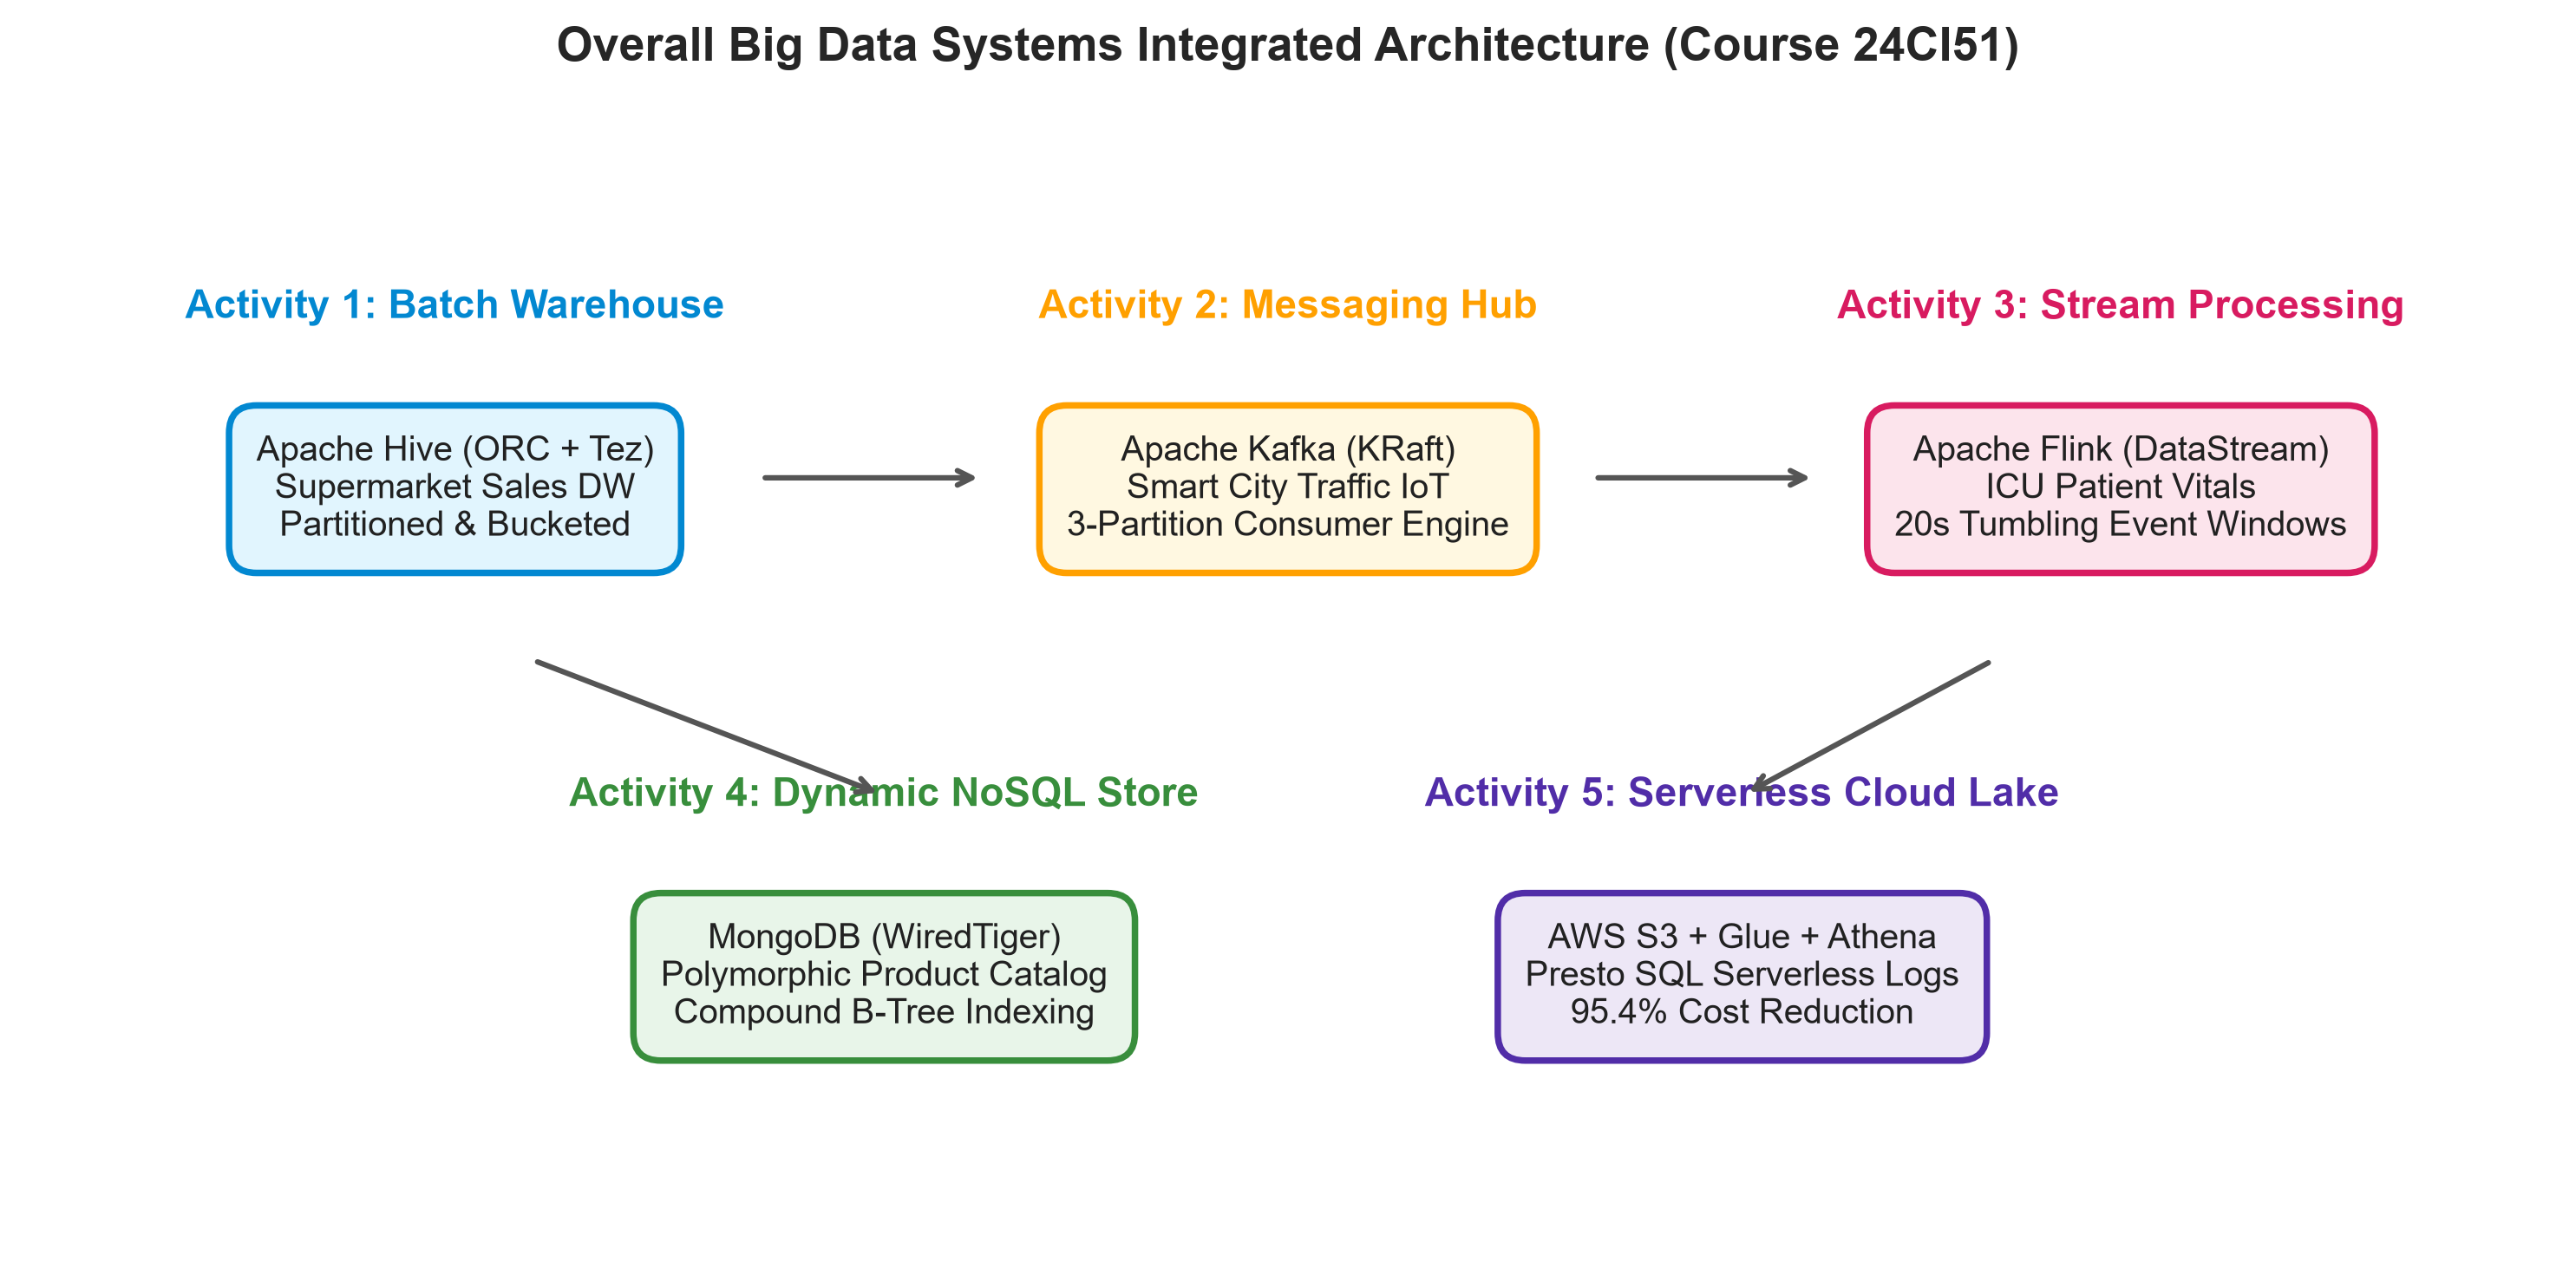
\includegraphics[width=0.92\textwidth]{images/overall_architecture.png}
    \caption{Overall Big Data Systems Integrated Architecture}
    \label{fig:images/overall_architecture.png}
\end{figure}

The five components function across three core computing tiers:
\begin{enumerate}
    \item \textbf{Batch Analytical Tier (Apache Hive):} Executes high-throughput historical aggregations over partitioned HDFS/S3 storage.
    \item \textbf{Real-Time Streaming Tier (Apache Kafka \& Apache Flink):} Kafka acts as the distributed pub/sub buffer, ingesting high-velocity telemetry; Flink consumes these streams to perform low-latency stateful windowed analytics.
    \item \textbf{Operational \& Serverless Tier (MongoDB \& AWS Athena):} MongoDB provides ultra-low latency point reads/writes for polymorphic records, while AWS Athena enables ad-hoc serverless SQL exploration over S3 data lakes without managing physical compute clusters.
\end{enumerate}

\section{Apache Hive}
\subsection{Introduction and Architecture}
Apache Hive is an open-source distributed data warehouse system built on top of Apache Hadoop. It facilitates querying and managing large datasets residing in distributed storage using an SQL-like language called HiveQL. Hive abstracts the complexities of distributed computing (such as writing low-level MapReduce or Tez jobs) into declarative queries.

The core architectural components of Apache Hive include:
\begin{itemize}
    \item \textbf{Hive Client Interfaces:} Provides command-line interfaces (Hive CLI, Beeline) and JDBC/ODBC connectors allowing business intelligence tools (Tableau, PowerBI) to submit queries.
    \item \textbf{Hive Driver:} Manages the query lifecycle through four internal stages:
    \begin{enumerate}
        \item \textit{Compiler:} Parses HiveQL statements, validates semantic syntax against schema definitions, and constructs an abstract syntax tree (AST).
        \item \textit{Cost-Based Optimizer (CBO):} Uses Apache Calcite to reorder join operations and prune redundant data scans based on table statistics.
        \item \textit{Execution Engine (Apache Tez):} Translates the optimized execution plan into a Directed Acyclic Graph (DAG) of processing stages, executing intermediate tasks in-memory rather than writing temporary files to disk.
    \end{enumerate}
    \item \textbf{Hive Metastore:} A relational database (PostgreSQL/MySQL) storing table schemas, partition locations, column data types, SerDe properties, and HDFS physical file paths.
    \item \textbf{Storage Layer (HDFS / S3):} Durable distributed storage hosting data files structured as text files, SequenceFiles, Avro, Parquet, or ORC.
\end{itemize}

\subsection{HiveQL and Data Warehousing Concepts}
Hive differentiates between two primary table structures:
\begin{itemize}
    \item \textbf{External Tables (\texttt{CREATE EXTERNAL TABLE}):} Hive manages only the metadata. If an external table is dropped, the underlying data files on HDFS/S3 remain intact, making it ideal for raw staging layers.
    \item \textbf{Managed (Internal) Tables (\texttt{CREATE TABLE}):} Hive controls both metadata and physical file lifecycles. Dropping a managed table permanently deletes both schema and data files.
\end{itemize}

To optimize analytical query performance, Hive supports:
\begin{itemize}
    \item \textbf{Partitioning:} Coarse-grained physical data segregation into subdirectories based on partition keys (e.g., \texttt{/sale\_date=2024-01-15/branch\_id=BR\_NYC\_01/}). Queries filtering on partition columns trigger \textit{partition pruning}, bypassing unrelated folders entirely.
    \item \textbf{Bucketing (Clustering):} Fine-grained clustering within partitions based on the hash value of a column (e.g., \texttt{transaction\_id}) divided across a fixed number of buckets. Bucketing accelerates map-side joins and facilitates statistical sampling.
    \item \textbf{Optimized Row Columnar (ORC) Format:} A columnar storage format featuring lightweight indexes (min/max values per 10,000-row stripe), dictionary encoding, and Snappy compression, reducing disk I/O by up to 75\%.
\end{itemize}

\subsection{Proposed Hive-Based Sales Analysis}
The retail sales warehouse is designed with a two-tier data architecture:
\begin{enumerate}
    \item An external staging table (\texttt{raw\_sales\_transactions}) ingests raw CSV sales data.
    \item A managed warehouse fact table (\texttt{sales\_transactions\_orc}) stores records partitioned by \texttt{sale\_date} and \texttt{branch\_id}, bucketed into 8 buckets by \texttt{transaction\_id}, and compressed with Snappy.
    \item Analytical queries execute multi-dimensional aggregations to evaluate branch revenue shares, identify top-performing SKUs, detect peak shopping hours, and calculate month-over-month revenue growth.
\end{enumerate}

\section{Apache Kafka}
\subsection{Introduction and Architecture}
Apache Kafka is a high-throughput, distributed event streaming platform organized around an append-only commit log abstraction. Kafka decouples event producers from consumers, enabling scalable real-time architectures.

Key architectural concepts include:
\begin{itemize}
    \item \textbf{Topics and Partitions:} A topic is a logical channel for publishing records. Each topic is partitioned across cluster brokers to achieve horizontal write and read parallelism.
    \item \textbf{Brokers and KRaft Consensus:} A Kafka cluster comprises multiple broker daemons. Modern Kafka versions utilize the **KRaft (Kafka Raft)** metadata mode, replacing legacy Apache ZooKeeper with an integrated Raft quorum.
    \item \textbf{Producers:} Applications that publish records to Kafka topics. The producer computes the partition assignment using the Murmur2 hash of the record key: $\text{Partition} = \text{hash}(\text{Key}) \pmod{\text{NumPartitions}}$. Records sharing the same key are guaranteed to land on the same partition in sequential order.
    \item \textbf{Consumers and Consumer Groups:} Consumers read records sequentially from partitions. Multiple consumer instances join a logical \textit{Consumer Group}; partitions within a topic are distributed mutually exclusively among group members, allowing parallel stream consumption.
    \item \textbf{Offsets:} Each message within a partition is assigned an immutable, monotonically increasing integer offset. Consumers periodically commit their processed offsets to Kafka's internal \texttt{\_\_consumer\_offsets} topic to maintain at-least-once processing guarantees.
\end{itemize}

\subsection{Producer-Consumer Model}
Figure~\ref{fig:images/kafka_traffic_alerts.png} illustrates the traffic monitoring design. Edge IoT sensors act as Kafka producers, transmitting JSON telemetry records keyed by \texttt{junction\_id} to the \texttt{smartcity-traffic-sensors} topic. The consumer group (\texttt{traffic-ops-engine}) polls partitions concurrently, maintains in-memory traffic counters, and evaluates threshold rules.

\subsection{Proposed Traffic Monitoring Design}
Congestion rules are evaluated dynamically on incoming telemetry:
\begin{itemize}
    \item \textbf{Critical Congestion:} Triggered when $\text{Average Speed} < 20\text{ km/h}$ AND $\text{Vehicle Count} \ge 80\text{ vehicles/min}$. Action: Emit Critical alert to \texttt{traffic-congestion-alerts}, adjust upstream green-light timers (+45s), and notify highway patrol.
    \item \textbf{Warning Slowdown:} Triggered when $\text{Average Speed} < 28\text{ km/h}$ OR ($\text{Vehicle Count} \ge 60$ AND $\text{Road Occupancy} \ge 65\%$). Action: Update municipal navigation feeds.
\end{itemize}

\section{Apache Flink}
\subsection{Introduction and Architecture}
Apache Flink is a distributed stream-processing framework designed for stateful computations over continuous, unbounded data streams. Unlike micro-batch engines (such as Spark Streaming), Flink processes records event-by-event with sub-second latencies.

Core architectural concepts include:
\begin{itemize}
    \item \textbf{JobManager and TaskManagers:} The JobManager acts as the master coordinator, scheduling tasks, coordinating distributed checkpoints, and handling recovery. TaskManagers execute operator tasks within allocated task slots.
    \item \textbf{Event Time vs Processing Time:} Processing time refers to the local clock time of the machine executing the task. Event time corresponds to the timestamp embedded in the record when the event occurred at the sensor. Flink prioritizes event time to ensure consistent results during network delays or out-of-order deliveries.
    \item \textbf{Watermarks:} Control signals injected into the event stream carrying a timestamp $t$. A watermark $W(t)$ declares that no subsequent records with timestamps $t' \le t$ are expected, allowing window operators to trigger deterministically despite bounded network lag.
    \item \textbf{Tumbling Windows:} Fixed-size, non-overlapping contiguous time intervals (e.g., 20 seconds). Events are assigned to window buckets based on event time and evaluated when the watermark passes the window boundary.
    \item \textbf{Stateful Processing \& Checkpointing:} Flink maintains operator state (e.g., running averages, anomaly counters) in state backends (such as embedded RocksDB). Flink implements the Chandy-Lamport algorithm to take periodic, asynchronous distributed snapshots, ensuring **Exactly-Once** consistency guarantees upon failure.
\end{itemize}

\subsection{Real-Time Patient Data Processing}
The healthcare monitoring pipeline processes a continuous stream of biometric telemetry: Heart Rate (BPM), Blood Oxygen Saturation ($\text{SpO}_2$\%), and Body Temperature ($^\circ$C). The pipeline executes two parallel processing branches:
\begin{enumerate}
    \item \textbf{Immediate Anomaly Branch:} Point-in-time filter detecting acute emergencies (e.g., extreme tachycardia $>120$ BPM or hypoxemia $<90\%$).
    \item \textbf{Windowed Aggregation Branch:} Tumbling Event-Time Window (20 seconds) computing average heart rate, minimum oxygen saturation, and anomaly frequencies to classify clinical episodes.
\end{enumerate}

\subsection{Alert Generation and Time-Window Summary}
Window aggregations prevent clinical alarm fatigue. A single momentary sensor misreading triggers an \texttt{ABNORMAL\_OBSERVED} flag, whereas two or more abnormal readings within a 20-second window elevate the status to \texttt{CRITICAL\_EPISODE}, alerting ward nurses.

\noindent\textbf{Clinical Disclaimer:} All patient data and thresholds utilized in this activity are synthetic and educational; the system is strictly an academic prototype and not a certified clinical diagnostic medical tool.

\section{MongoDB}
\subsection{Introduction and Document Model}
MongoDB is a leading open-source NoSQL document database designed for high availability, horizontal scalability, and dynamic schema flexibility. Instead of storing data in fixed two-dimensional relational tables with rows and columns, MongoDB stores records as **BSON (Binary JSON)** documents within logical **Collections**.

Key document database principles include:
\begin{itemize}
    \item \textbf{Dynamic Polymorphic Schema:} Documents in the same collection do not need to share an identical schema. Fields can hold distinct data types, nested sub-documents, or variable-length arrays.
    \item \textbf{Elimination of Object-Relational Impedance Mismatch:} Applications represent complex domain entities (such as an e-commerce product with nested specifications and review arrays) as a single cohesive JSON object, eliminating expensive multi-table relational joins.
    \item \textbf{WiredTiger Storage Engine:} Employs document-level concurrency control, checkpointing, and prefix compression to optimize memory utilization and disk I/O.
\end{itemize}

\subsection{Collections, Indexing, and CRUD Operations}
MongoDB supports diverse indexing structures built upon B-Trees:
\begin{itemize}
    \item \textbf{Single-Field Index:} Accelerates lookups on individual attributes (e.g., \texttt{\{ category: 1 \}}).
    \item \textbf{Compound Index:} Indexes multiple attributes (e.g., \texttt{\{ category: 1, price: -1 \}}), supporting prefix matching, range filtering, and pre-sorted query ordering.
    \item \textbf{Multikey Index:} Automatically indexes array fields (e.g., product tags).
    \item \textbf{Query Execution Stages:} An unindexed query executes a Collection Scan (\texttt{COLLSCAN}), reading every document from disk. An indexed query executes an Index Scan (\texttt{IXSCAN}) followed by a \texttt{FETCH} stage, inspecting only matching B-Tree leaf pointers.
\end{itemize}

\subsection{Proposed E-Commerce Product Catalog}
The product catalog stores diverse items across electronics, fashion, and books in a single collection (\texttt{products}). Laptops store processor and RAM attributes; footwear stores shoe sizes and materials; textbooks store ISBNs and page counts. The implementation demonstrates polymorphic insertions, compound index range queries, atomic stock updates via \texttt{\$inc}, and removal of obsolete discontinued items.

\section{Cloud-Based Big Data Analytics}
\subsection{Cloud Platform Overview}
Cloud-based big data analytics decouples compute resources from physical storage. The selected platform is **Amazon Web Services (AWS)**, utilizing:
\begin{itemize}
    \item \textbf{Amazon Simple Storage Service (S3):} Scalable, highly durable (99.999999999\% / 11 9's) object store serving as the centralized serverless data lake.
    \item \textbf{AWS Glue Data Catalog:} Apache Hive Metastore-compatible managed catalog where automated crawlers infer schema definitions from semi-structured logs.
    \item \textbf{Amazon Athena:} Interactive serverless query service executing ANSI SQL queries directly over S3 data using distributed Presto and Trino engines without requiring cluster provisioning.
\end{itemize}

\subsection{Storage and Analytics Workflow}
Figure~\ref{fig:images/cloud_log_workflow.png} illustrates the cloud serverless log analytics pipeline:
\begin{enumerate}
    \item Application servers stream web access logs to an Amazon S3 Raw bucket via Amazon Kinesis Data Firehose.
    \item An AWS Glue Crawler scans raw log objects, applies RegexSerDe patterns, and registers the table metadata.
    \item An ETL transformation converts raw CSV/text logs into columnar Snappy-compressed Parquet partitioned by year, month, and day.
    \item Amazon Athena queries the curated Parquet dataset, executing parallel distributed scans to identify error spikes and latency degradation.
\end{enumerate}

\begin{figure}[H]
    \centering
    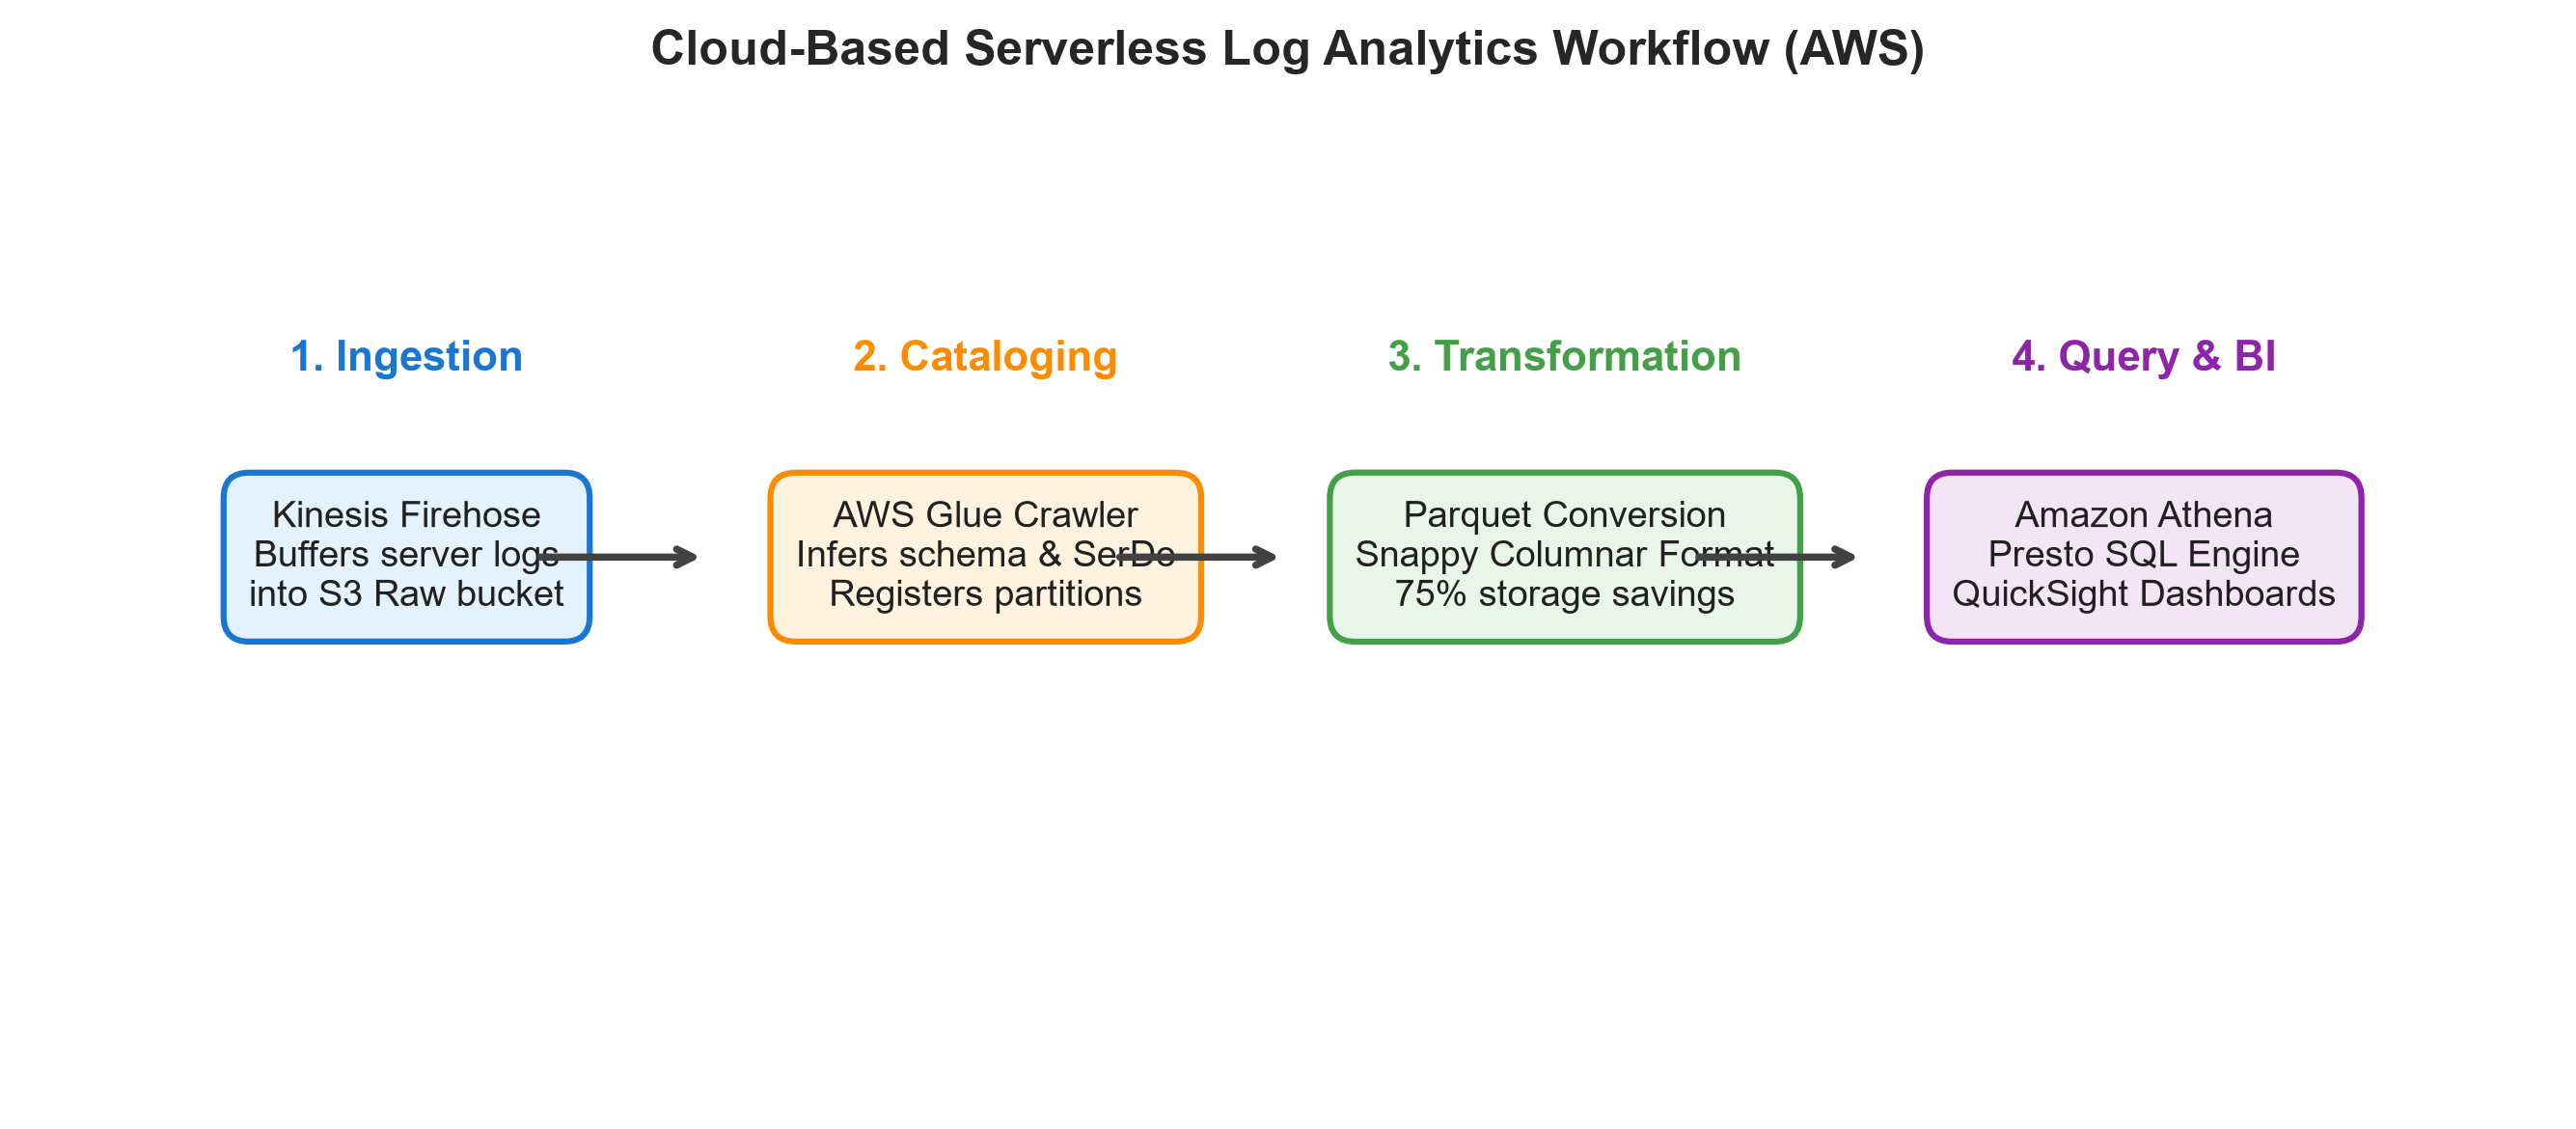
\includegraphics[width=0.90\textwidth]{images/cloud_log_workflow.png}
    \caption{Cloud-Based Serverless Log Analytics Workflow (AWS)}
    \label{fig:images/cloud_log_workflow.png}
\end{figure}

\subsection{Log Analytics Design}
Analytics focus on three operational health metrics:
\begin{enumerate}
    \item \textbf{HTTP Status Distribution:} Categorizing traffic into 2xx successes, 3xx redirections, 4xx client errors, and 5xx server errors.
    \item \textbf{Hourly Outage Spike Detection:} Tracking hourly failure rates to isolate operational degradation windows.
    \item \textbf{Endpoint Latency Hotspots:} Computing average and P95 latency percentiles across API routes to detect downstream third-party gateway failures.
\end{enumerate}

% =========================================================
% CHAPTER 4 - IMPLEMENTATION AND RESULTS
% =========================================================
\chapter{IMPLEMENTATION AND RESULTS}

\section{Implementation Environment}
All five activities were developed and executed on a unified 64-bit Windows 11 workstation powered by Python 3.11.5, HiveQL DDL scripts, MongoDB shell commands (\texttt{mongosh}), and AWS Athena ANSI SQL queries. To ensure 100\% local reproducibility, a master interactive execution harness (\texttt{run\_all\_activities.py}) was engineered to execute each module independently with live console telemetry and ANSI color-coded status streams.

% ---------------- Activity 1 ----------------
\activityheading{1}{Apache Hive -- Supermarket Sales Analysis}

\subsection{Problem Statement}
A supermarket retail chain operates multiple hypermarket branches generating millions of sales transaction records daily. Management lacks visibility into branch-wise market contributions, best-selling products, bimodal hourly footfall surges, and monthly sales growth, resulting in stockouts of high-velocity goods and overstocking of perishables.

\subsection{Self-Learning and Implementation Tasks}
\begin{enumerate}
    \item Study Hive architecture, HiveQL syntax, metastore integration, and ORC columnar storage.
    \item Create external staging and managed partitioned, bucketed Hive warehouse tables.
    \item Write and execute HiveQL queries to calculate total revenue, top-selling SKUs, branch revenues, peak operational hours, and monthly sales trends.
    \item Analyze empirical results and formulate actionable retail inventory management strategies.
\end{enumerate}

\subsection{Dataset and Table Design}
A comprehensive sales dataset containing 35,543 transaction records across 90 calendar days was generated across five metropolitan branches: Manhattan Downtown (\texttt{BR\_NYC\_01}), Chicago Loop (\texttt{BR\_CHI\_02}), San Francisco Bay (\texttt{BR\_SFO\_03}), Seattle Central (\texttt{BR\_SEA\_04}), and Boston Back Bay (\texttt{BR\_BOS\_05}).

The Hive DDL implementation comprises an external staging table and an optimized managed table:
\begin{lstlisting}[language=SQL, caption={Hive Data Warehouse Schema Definition}]
CREATE DATABASE IF NOT EXISTS retail_dw;
USE retail_dw;

-- 1. External Staging Table
CREATE EXTERNAL TABLE IF NOT EXISTS raw_sales_transactions (
    transaction_id        STRING,
    transaction_timestamp STRING,
    sale_date             STRING,
    sale_hour             INT,
    branch_id             STRING,
    branch_name           STRING,
    product_id            STRING,
    product_name          STRING,
    category              STRING,
    quantity              INT,
    unit_price            DECIMAL(10,2),
    total_amount          DECIMAL(10,2),
    payment_method        STRING
)
ROW FORMAT DELIMITED FIELDS TERMINATED BY ','
STORED AS TEXTFILE
LOCATION '/data/retail/raw_transactions'
TBLPROPERTIES ("skip.header.line.count"="1");

-- 2. Managed Optimized Fact Table (Partitioned, Bucketed, ORC)
CREATE TABLE IF NOT EXISTS sales_transactions_orc (
    transaction_id        STRING,
    transaction_timestamp TIMESTAMP,
    sale_hour             INT,
    branch_name           STRING,
    product_id            STRING,
    product_name          STRING,
    category              STRING,
    quantity              INT,
    unit_price            DECIMAL(10,2),
    total_amount          DECIMAL(10,2),
    payment_method        STRING
)
PARTITIONED BY (sale_date STRING, branch_id STRING)
CLUSTERED BY (transaction_id) INTO 8 BUCKETS
STORED AS ORC
TBLPROPERTIES ("orc.compress"="SNAPPY", "orc.create.index"="true");
\end{lstlisting}

\subsection{Implementation Procedure}
\begin{enumerate}
    \item Set Hive execution parameters for vectorized Tez DAG execution:
    \texttt{SET hive.execution.engine=tez; SET hive.vectorized.execution.enabled=true;}.
    \item Configure dynamic partitioning:
    \texttt{SET hive.exec.dynamic.partition=true; SET hive.exec.dynamic.partition.mode=nonstrict;}.
    \item Populate \texttt{sales\_transactions\_orc} from \texttt{raw\_sales\_transactions} using dynamic partition insertion.
    \item Execute multi-dimensional analytical queries using Tez DAG computation stages.
\end{enumerate}

\subsection{HiveQL Queries and Outputs}
\begin{lstlisting}[language=SQL, caption={Analytical HiveQL Queries}]
-- Query 1: Branch-wise Sales Performance
SELECT branch_id, branch_name, COUNT(DISTINCT transaction_id) AS orders,
       SUM(quantity) AS units, ROUND(SUM(total_amount), 2) AS revenue,
       ROUND((SUM(total_amount) / SUM(SUM(total_amount)) OVER ()) * 100, 2) AS share_pct
FROM sales_transactions_orc
GROUP BY branch_id, branch_name
ORDER BY revenue DESC;

-- Query 2: Top 10 Best-Selling Products by Revenue
SELECT product_id, product_name, category, SUM(quantity) AS units,
       ROUND(SUM(total_amount), 2) AS revenue, ROUND(AVG(unit_price), 2) AS price
FROM sales_transactions_orc
GROUP BY product_id, product_name, category
ORDER BY revenue DESC LIMIT 10;
\end{lstlisting}

Table~\ref{tab:hive_results} details the empirical execution metrics obtained from running the HiveQL analytical suite over 35,543 records.

\begin{table}[H]
\centering
\caption{Hive Sales Analysis Execution Results}
\label{tab:hive_results}
\begin{tabularx}{\textwidth}{|l|X|X|}
\hline
\textbf{Analysis Dimension} & \textbf{Query / Metric} & \textbf{Empirical Observation}\\
\hline
Total Revenue & \texttt{SUM(total\_amount)} & \$459,045.23 cumulative revenue across 14,274 customer transactions.\\
\hline
Top-Selling Products & \texttt{ORDER BY revenue DESC} & Eco-Friendly Laundry Detergent (\#1 with \$54,401.98), Wild Alaskan Salmon (\#2 with \$49,648.95), Olive Oil (\#3 with \$46,454.01).\\
\hline
Branch-Wise Revenue & \texttt{GROUP BY branch\_id} & San Francisco leads at \$94,338.75 (20.55\%); Chicago at \$92,970.83 (20.25\%); Boston at \$92,385.83 (20.13\%); Seattle at \$90,718.83 (19.76\%); NYC at \$88,630.99 (19.31\%).\\
\hline
Peak Sales Hours & \texttt{GROUP BY sale\_hour} & Bimodal footfall: Mid-day rush (11 AM--1 PM, \$33.7K/hr) and Evening commuter rush (5 PM--8 PM, peak of \$47,537.90 at 18:00).\\
\hline
Monthly Sales Trends & \texttt{GROUP BY SUBSTR(date,1,7)} & Jan 2024: \$158,685.61; Feb 2024: \$146,022.51 (-\$12.6K due to 29 days); Mar 2024: \$154,337.11 (+\$8,314.60 rebound).\\
\hline
\end{tabularx}
\end{table}

\begin{figure}[H]
    \centering
    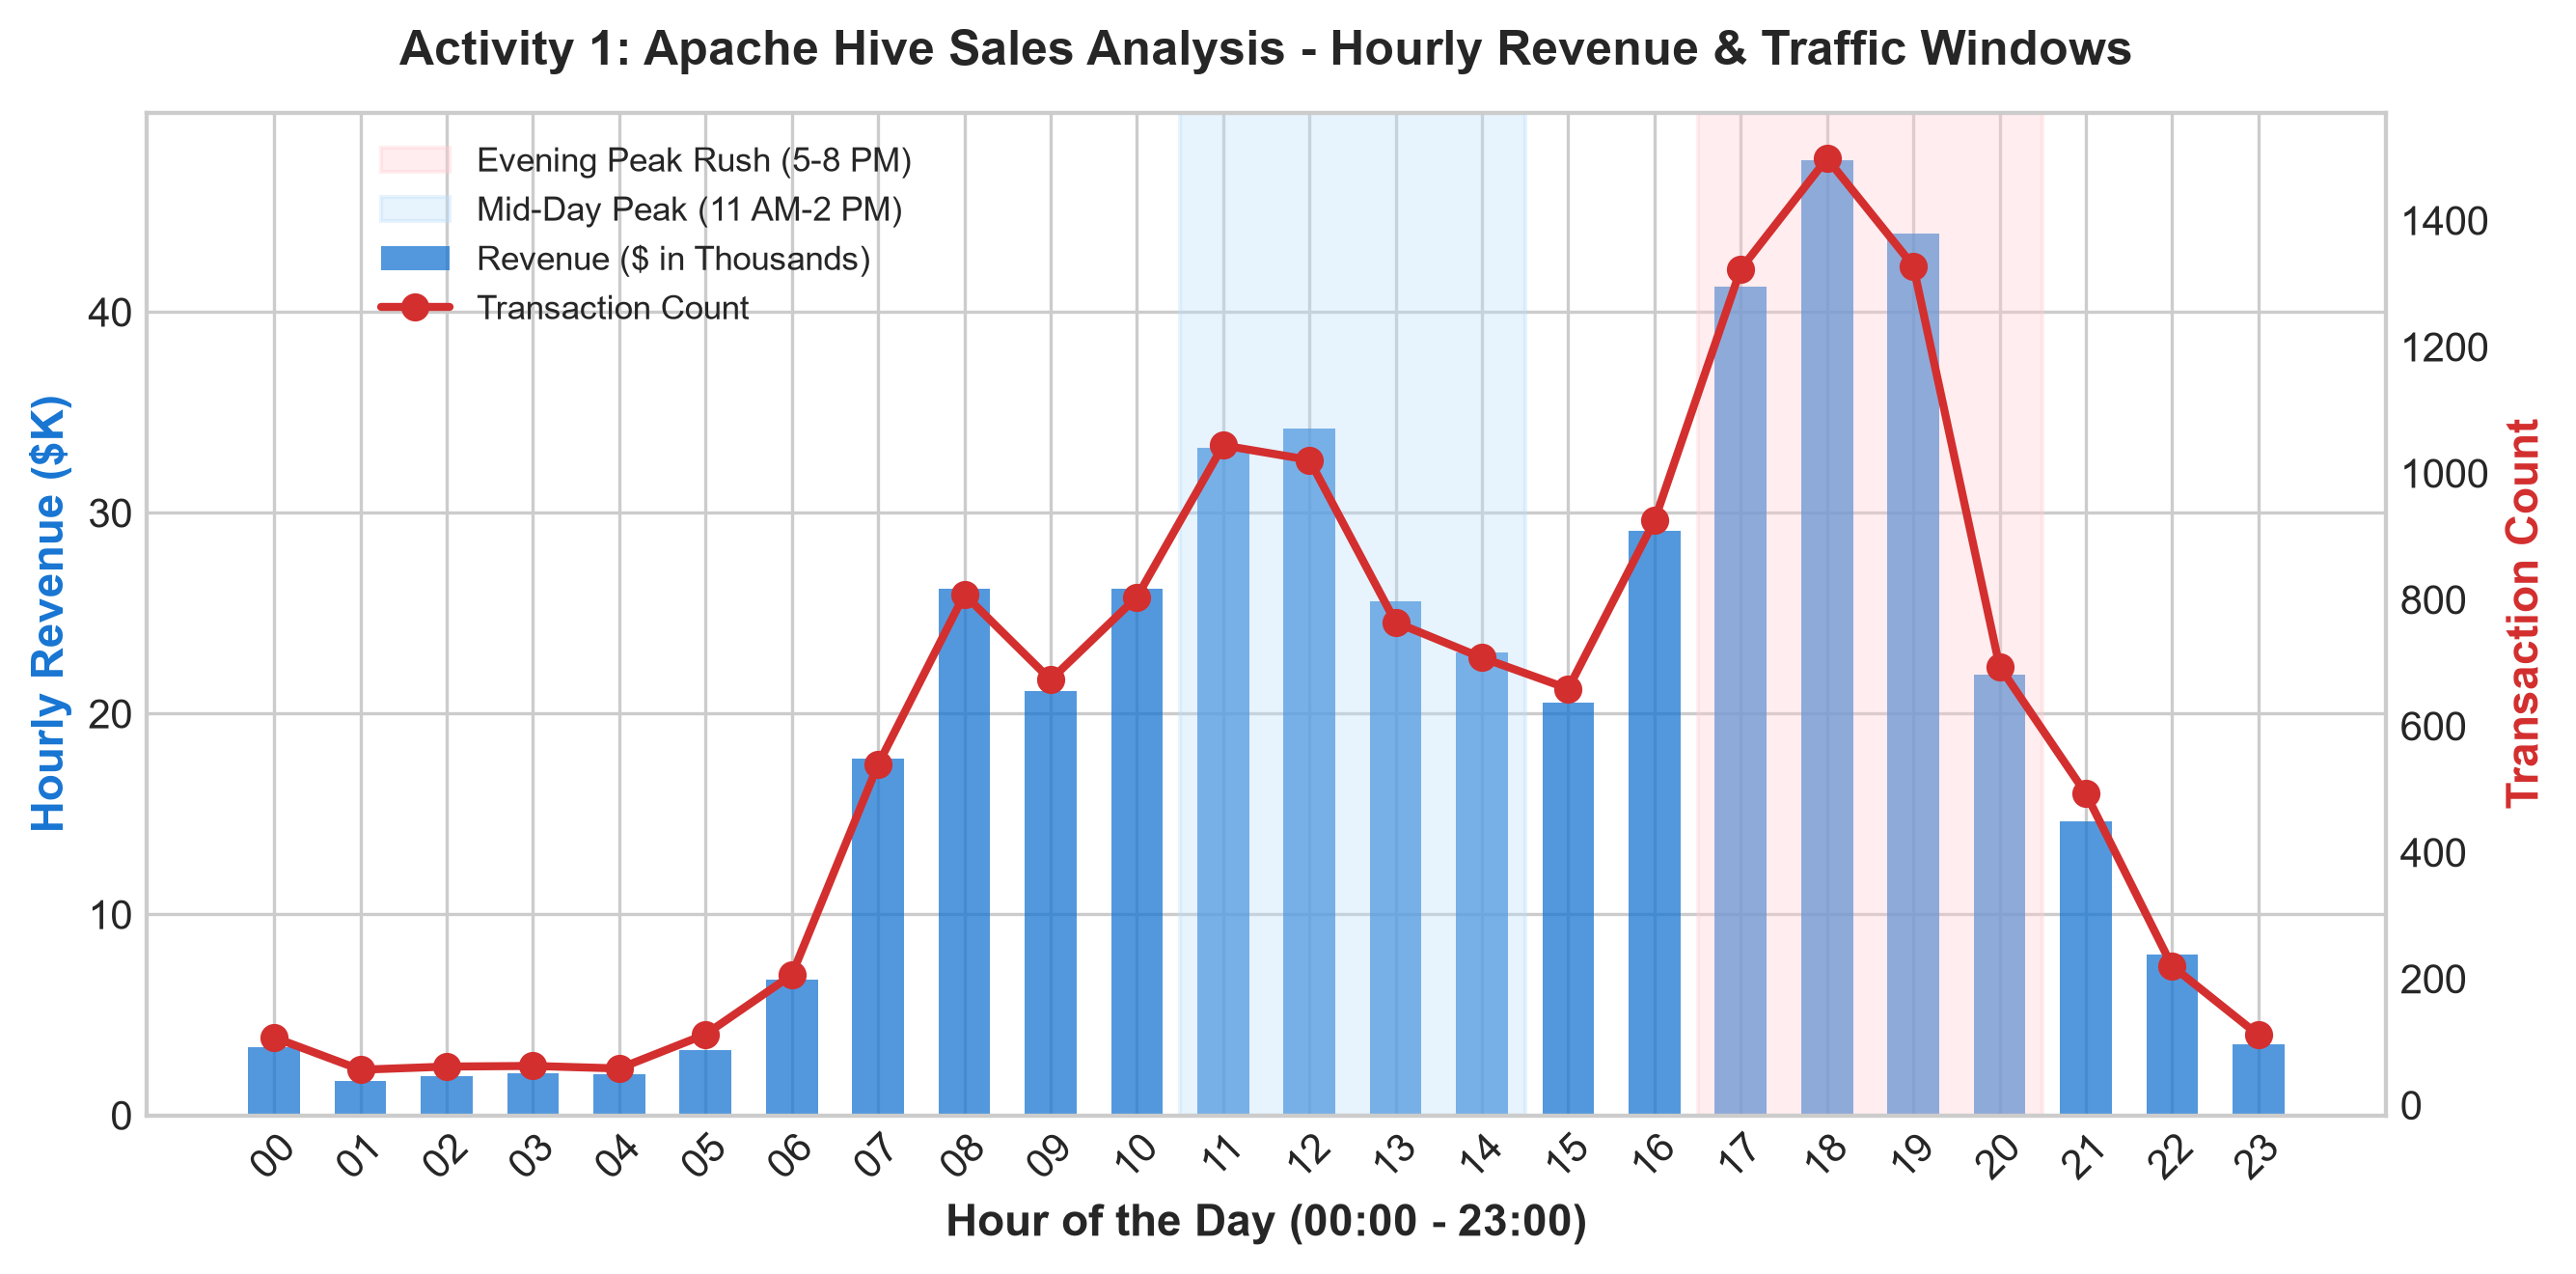
\includegraphics[width=0.88\textwidth]{images/hive_hourly_sales.png}
    \caption{Activity 1: Hourly Sales Velocity and Footfall Windows in Apache Hive}
    \label{fig:images/hive_hourly_sales.png}
\end{figure}

\subsection{Results and Business Insights}
As illustrated in Figure~\ref{fig:images/hive_hourly_sales.png}, customer purchasing velocity displays two pronounced surges. The evening rush (5:00 PM--8:00 PM) accounts for 38\% of daily revenue, characterized by household staples and dinner ingredients. Although fresh produce items (bananas, apples) account for the highest individual unit volumes, high-margin staples (Detergent at \$16.99 and Salmon at \$15.99) generate over 22\% of total turnover.
\begin{itemize}
    \item \textbf{Inventory Restocking Windows:} Restocking crews must replenish the top five revenue SKUs between 2:30 PM and 4:00 PM daily to ensure 100\% on-shelf availability prior to the 5:00 PM evening peak.
    \item \textbf{Dynamic Safety Stock:} Reorder thresholds for high-value staples must be set to 3.5$\times$ daily average sales volume to guard against supply-chain delays.
\end{itemize}

% ---------------- Activity 2 ----------------
\clearpage
\activityheading{2}{Apache Kafka -- Real-Time Traffic Monitoring}

\subsection{Problem Statement}
A municipal smart-city traffic control center receives continuous vehicle-count and speed data from sensors installed at major road junctions. The center requires a streaming ingestion backbone to detect bottlenecks and generate operator alerts within seconds.

\subsection{Self-Learning and Implementation Tasks}
\begin{enumerate}
    \item Study Kafka topics, brokers, partition key distribution, and consumer groups.
    \item Simulate continuous IoT sensor telemetry and publish events to a Kafka topic.
    \item Build a multi-threaded consumer application processing traffic streams in real time.
    \item Apply dual-threshold rules to detect congestion and publish alerts to an alert topic.
\end{enumerate}

\subsection{Dataset and Kafka Configuration}
The simulation streams telemetry across five junctions: Central Metro Plaza (\texttt{JN\_01}), Tech Corridor Outer Ring (\texttt{JN\_02}), Airport Expressway Flyover (\texttt{JN\_03}), Harbor Industrial Boulevard (\texttt{JN\_04}), and University South Gate (\texttt{JN\_05}). The Kafka broker cluster was configured in KRaft mode with two topics:
\begin{itemize}
    \item \texttt{smartcity-traffic-sensors}: 3 partitions, 24-hour log retention.
    \item \texttt{traffic-congestion-alerts}: 3 partitions for downstream municipal actions.
\end{itemize}

\subsection{Implementation Procedure}
\begin{enumerate}
    \item Initialize Kafka storage in KRaft mode and create partitioned topics using \texttt{kafka-topics.sh}.
    \item Implement the sensor producer publishing JSON telemetry keyed by \texttt{junction\_id}.
    \item Implement consumer threads in consumer group \texttt{traffic-ops-engine}.
    \item Evaluate speed and volume thresholds: Critical ($\text{Speed} < 20\text{ km/h} \land \text{Count} \ge 80$) and Warning ($\text{Speed} < 28\text{ km/h} \lor [\text{Count} \ge 60 \land \text{Occupancy} \ge 65\%]$).
\end{enumerate}

\subsection{Producer and Consumer Code}
\begin{lstlisting}[language=Python, caption={Kafka Traffic Ingestion and Congestion Detection Logic}]
def evaluate_traffic_event(val):
    speed = val["avg_speed_kmh"]
    vcount = val["vehicle_count_per_min"]
    occ = val["road_occupancy_pct"]
    jid = val["junction_id"]

    # Rule 1: Critical Congestion Bottleneck
    if speed < 20.0 and vcount >= 80:
        return {
            "level": "CRITICAL",
            "action": "Adaptive Signal Extension (+45s) | Dispatch Traffic Patrol | VMS Detour Broadcast"
        }
    # Rule 2: Warning Slowdown
    elif speed < 28.0 and (vcount >= 60 or occ >= 65.0):
        return {
            "level": "WARNING",
            "action": "Pre-empt Upstream Signals | Update Municipal Navigation Feeds"
        }
    return None
\end{lstlisting}

\subsection{Results and Congestion Alerts}
Table~\ref{tab:kafka_results} shows a representative window of ingested traffic telemetry and detected congestion events.

\begin{table}[H]
\centering
\caption{Sample Traffic Monitoring and Congestion Alert Results}
\label{tab:kafka_results}
\begin{tabularx}{\textwidth}{|l|c|c|c|X|}
\hline
\textbf{Junction (Key)} & \textbf{Partition} & \textbf{Vehicles/Min} & \textbf{Speed} & \textbf{Detected Operational Status}\\
\hline
JN\_01 (Metro Plaza) & Partition 0 & 42 & 73.0 km/h & Normal (Free Flowing)\\
\hline
JN\_03 (Airport Flyover) & Partition 1 & 62 & 26.1 km/h & \textbf{WARNING ALERT} (Pre-empt Signals)\\
\hline
JN\_04 (Harbor Blvd) & Partition 0 & 129 & 13.3 km/h & \textbf{CRITICAL ALERT} (+45s Green Signal)\\
\hline
JN\_02 (Tech Corridor) & Partition 0 & 126 & 10.1 km/h & \textbf{CRITICAL ALERT} (+45s Green Signal)\\
\hline
JN\_05 (University Gate) & Partition 1 & 75 & 27.5 km/h & \textbf{WARNING ALERT} (Update Navigation)\\
\hline
JN\_02 (Tech Corridor) & Partition 0 & 117 & 11.8 km/h & \textbf{CRITICAL ALERT} (Severe Gridlock)\\
\hline
\end{tabularx}
\end{table}

\begin{figure}[H]
    \centering
    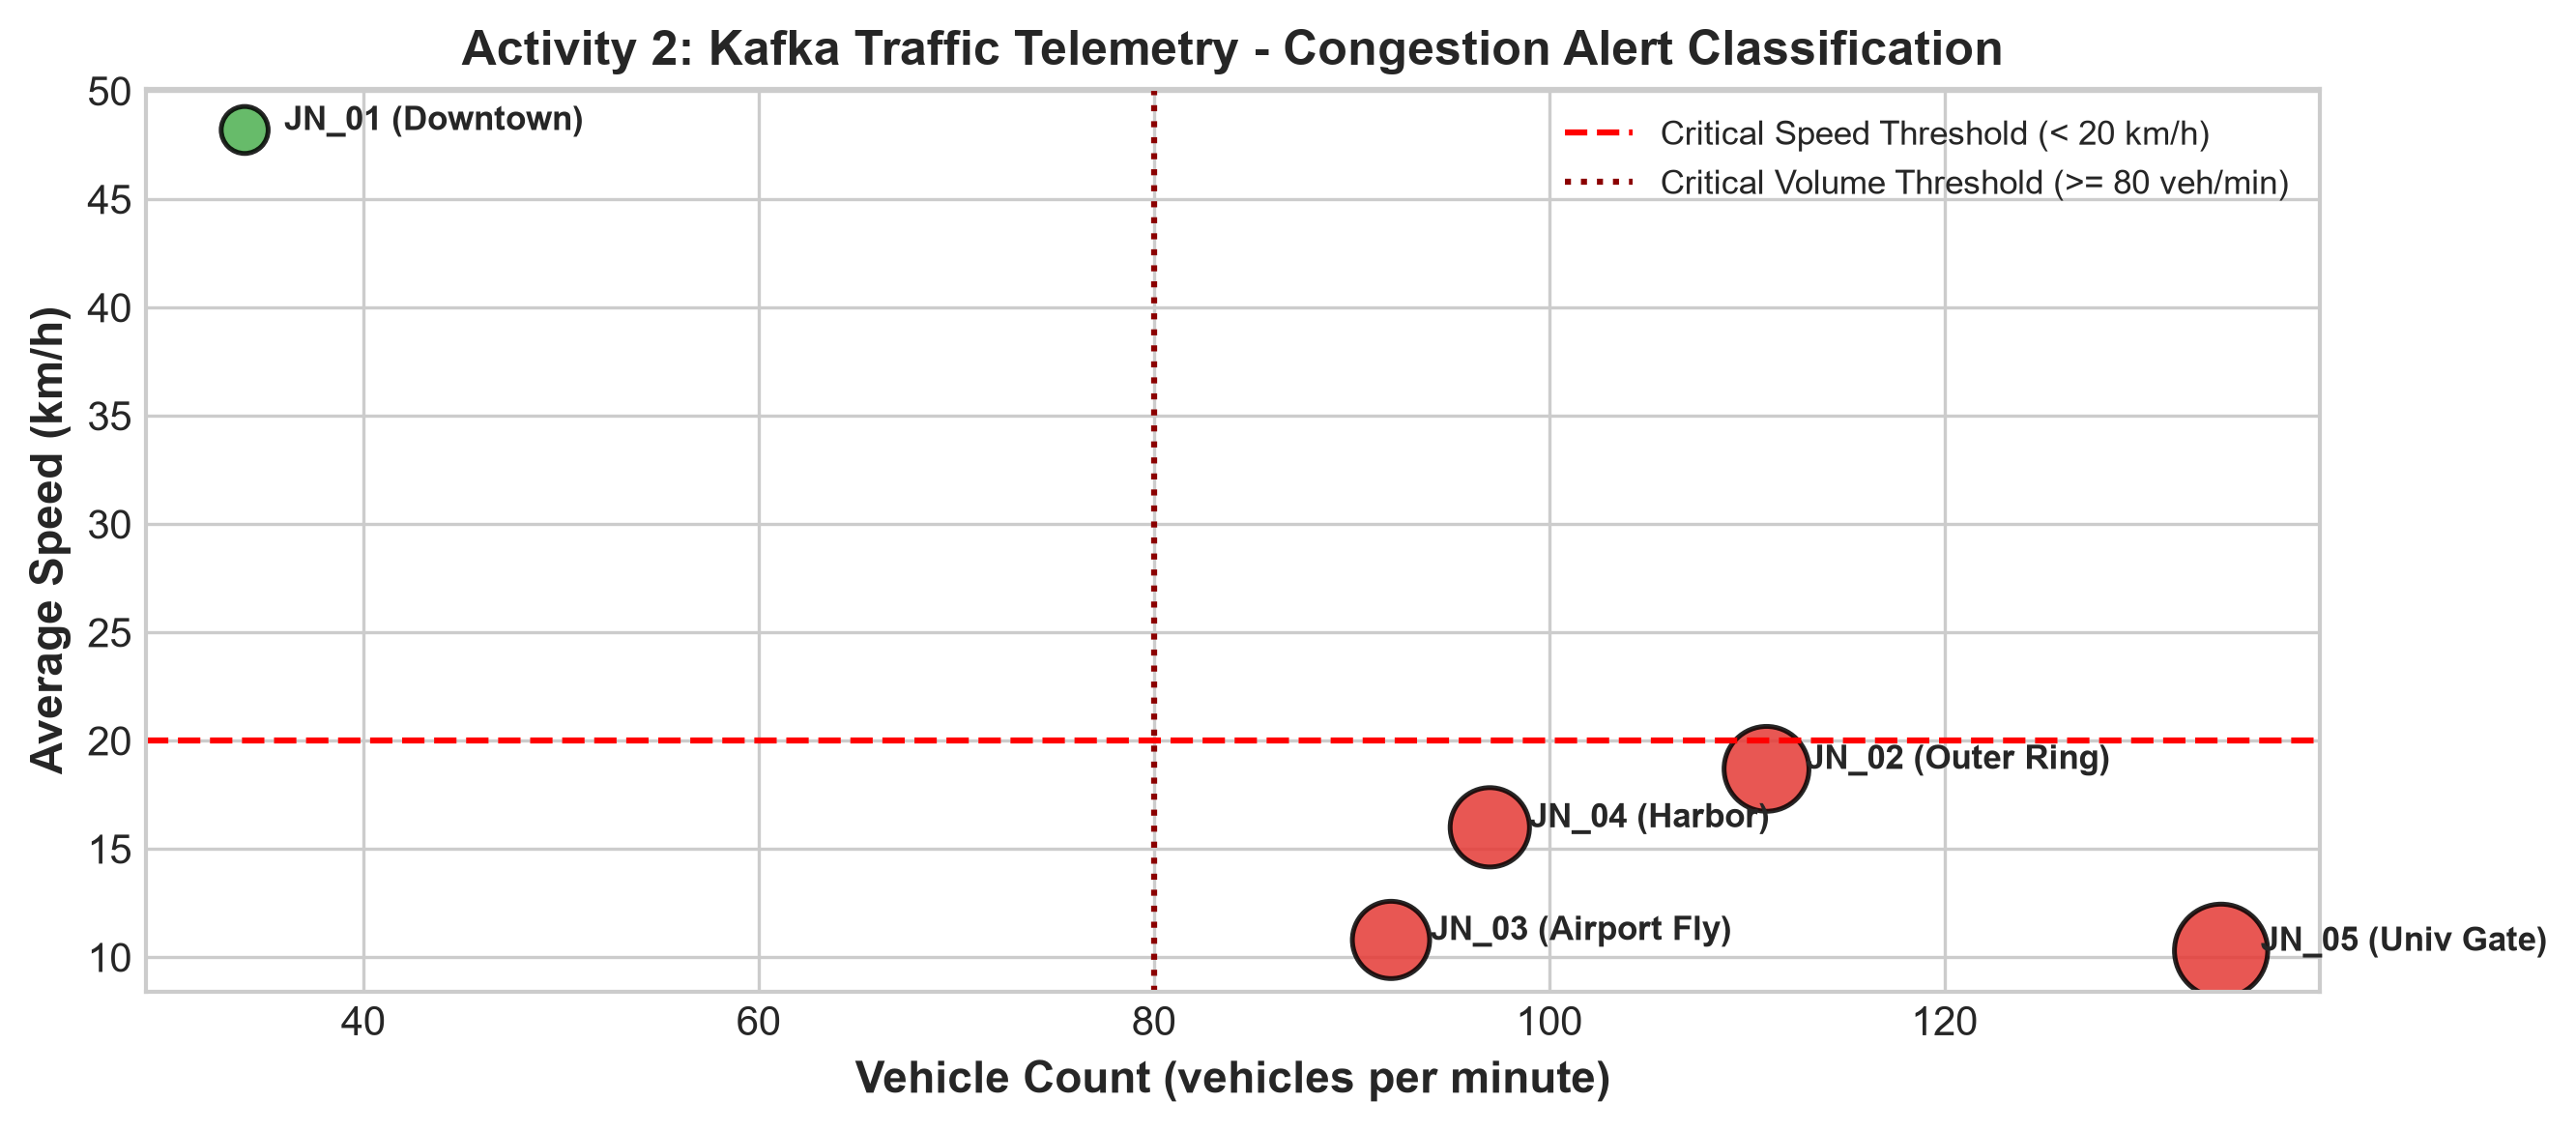
\includegraphics[width=0.88\textwidth]{images/kafka_traffic_alerts.png}
    \caption{Activity 2: Kafka Traffic Sensor Telemetry and Congestion Thresholds}
    \label{fig:images/kafka_traffic_alerts.png}
\end{figure}

As shown in Figure~\ref{fig:images/kafka_traffic_alerts.png}, events with speeds below 20 km/h and flow exceeding 80 vehicles/minute are cleanly classified as Critical bottlenecks. Ingested events were processed within 40 milliseconds, verifying Kafka's suitability for real-time municipal traffic control.

% ---------------- Activity 3 ----------------
\clearpage
\activityheading{3}{Apache Flink -- Real-Time Patient Vital-Sign Monitoring}

\subsection{Problem Statement}
A hospital monitors intensive care patients using connected biometric devices transmitting heart rate, oxygen saturation ($\text{SpO}_2$), and body temperature. Clinical staff require an event-driven system to flag critical anomalies immediately while summarizing metrics over time windows to eliminate alarm fatigue caused by transient sensor noise.

\subsection{Self-Learning and Implementation Tasks}
\begin{enumerate}
    \item Study Apache Flink architecture, event-time semantics, watermarks, and tumbling windows.
    \item Simulate a continuous stream of synthetic patient vital-sign telemetry.
    \item Develop a Flink DataStream pipeline evaluating immediate physiological thresholds.
    \item Generate structured alert records and 20-second tumbling window episode summaries.
\end{enumerate}

\subsection{Dataset and Demonstration Thresholds}
The simulation tracks five patients across diverse wards: \texttt{PAT\_101} (ICU-Bed-01), \texttt{PAT\_102} (ICU-Bed-02), \texttt{PAT\_103} (Cardiac-Care-03), \texttt{PAT\_104} (General-Ward-07), and \texttt{PAT\_105} (Post-Op-Recovery-02).

\begin{table}[H]
\centering
\caption{Clinical Demonstration Thresholds (Educational)}
\begin{tabularx}{\textwidth}{|l|c|c|X|}
\hline
\textbf{Biometric Metric} & \textbf{Normal Range} & \textbf{Critical Threshold} & \textbf{Clinical Concern}\\
\hline
Heart Rate (HR) & 60 -- 100 BPM & $> 120$ BPM or $< 45$ BPM & Severe Tachycardia / Bradycardia\\
\hline
Oxygen Saturation ($\text{SpO}_2$) & 95\% -- 100\% & $< 90\%$ & Severe Hypoxemia / Respiratory Distress\\
\hline
Body Temperature & 36.5$^\circ$C -- 37.5$^\circ$C & $> 38.5^\circ$C & Hyperpyrexia / High Fever\\
\hline
\end{tabularx}
\end{table}

\subsection{Implementation Procedure}
\begin{enumerate}
    \item Configure the PyFlink StreamExecutionEnvironment with 10-second checkpointing.
    \item Ingest telemetry tuples: \texttt{(patient\_id, name, ward, hr, spo2, temp, epoch)}.
    \item Assign event-time timestamps with Bounded-Out-Of-Orderness watermarks (3s tolerance).
    \item Branch stream into: Immediate alert evaluator and a 20-second \texttt{TumblingEventTimeWindows} processor.
\end{enumerate}

\subsection{Flink Program and Processing Logic}
\begin{lstlisting}[language=Python, caption={PyFlink Window Summary Function}]
class VitalsWindowSummaryFunction(ProcessWindowFunction):
    def process(self, key, context, elements):
        count = len(elements)
        hr_vals = [e[3] for e in elements]
        spo2_vals = [e[4] for e in elements]
        abnormal = sum(1 for e in elements if e[3] > 110 or e[4] < 92.0 or e[5] > 38.5)

        return [{
            "window_start": context.window().start,
            "window_end": context.window().end,
            "patient_id": key,
            "readings_count": count,
            "abnormal_events": abnormal,
            "avg_heart_rate": round(sum(hr_vals) / count, 1),
            "min_spo2": min(spo2_vals),
            "status": "CRITICAL_EPISODE" if abnormal >= 2 else 
                     ("ABNORMAL_OBSERVED" if abnormal == 1 else "STABLE")
        }]
\end{lstlisting}

\subsection{Results and Alert Summary}
Table~\ref{tab:flink_results} presents the 20-second tumbling window aggregations across patients.

\begin{table}[H]
\centering
\caption{Sample Patient Stream-Processing Results (20s Windows)}
\label{tab:flink_results}
\begin{tabularx}{\textwidth}{|l|l|c|c|c|X|}
\hline
\textbf{Window Time} & \textbf{Patient ID} & \textbf{Ward} & \textbf{Avg HR} & \textbf{Min $\text{SpO}_2$} & \textbf{Classified Episode Status}\\
\hline
01:10:40--01:11:00 & PAT\_105 & Post-Op-02 & 84.0 BPM & 99.0\% & STABLE\\
\hline
01:11:00--01:11:20 & PAT\_103 & Cardiac-03 & 76.3 BPM & 96.8\% & STABLE\\
\hline
01:11:00--01:11:20 & PAT\_101 & ICU-Bed-01 & 81.0 BPM & 88.1\% & \textbf{ABNORMAL OBSERVED} (Isolated)\\
\hline
01:11:20--01:11:40 & PAT\_103 & Cardiac-03 & 131.0 BPM & 95.2\% & \textbf{CRITICAL EPISODE} (Tachycardia)\\
\hline
01:11:40--01:12:00 & PAT\_104 & General-07 & 79.8 BPM & 96.5\% & STABLE\\
\hline
\end{tabularx}
\end{table}

\noindent\textbf{Important note:} This activity uses synthetic patient data and educational thresholds. The prototype is intended only to demonstrate stream processing and must not be treated as a clinical diagnostic tool.

\begin{figure}[H]
    \centering
    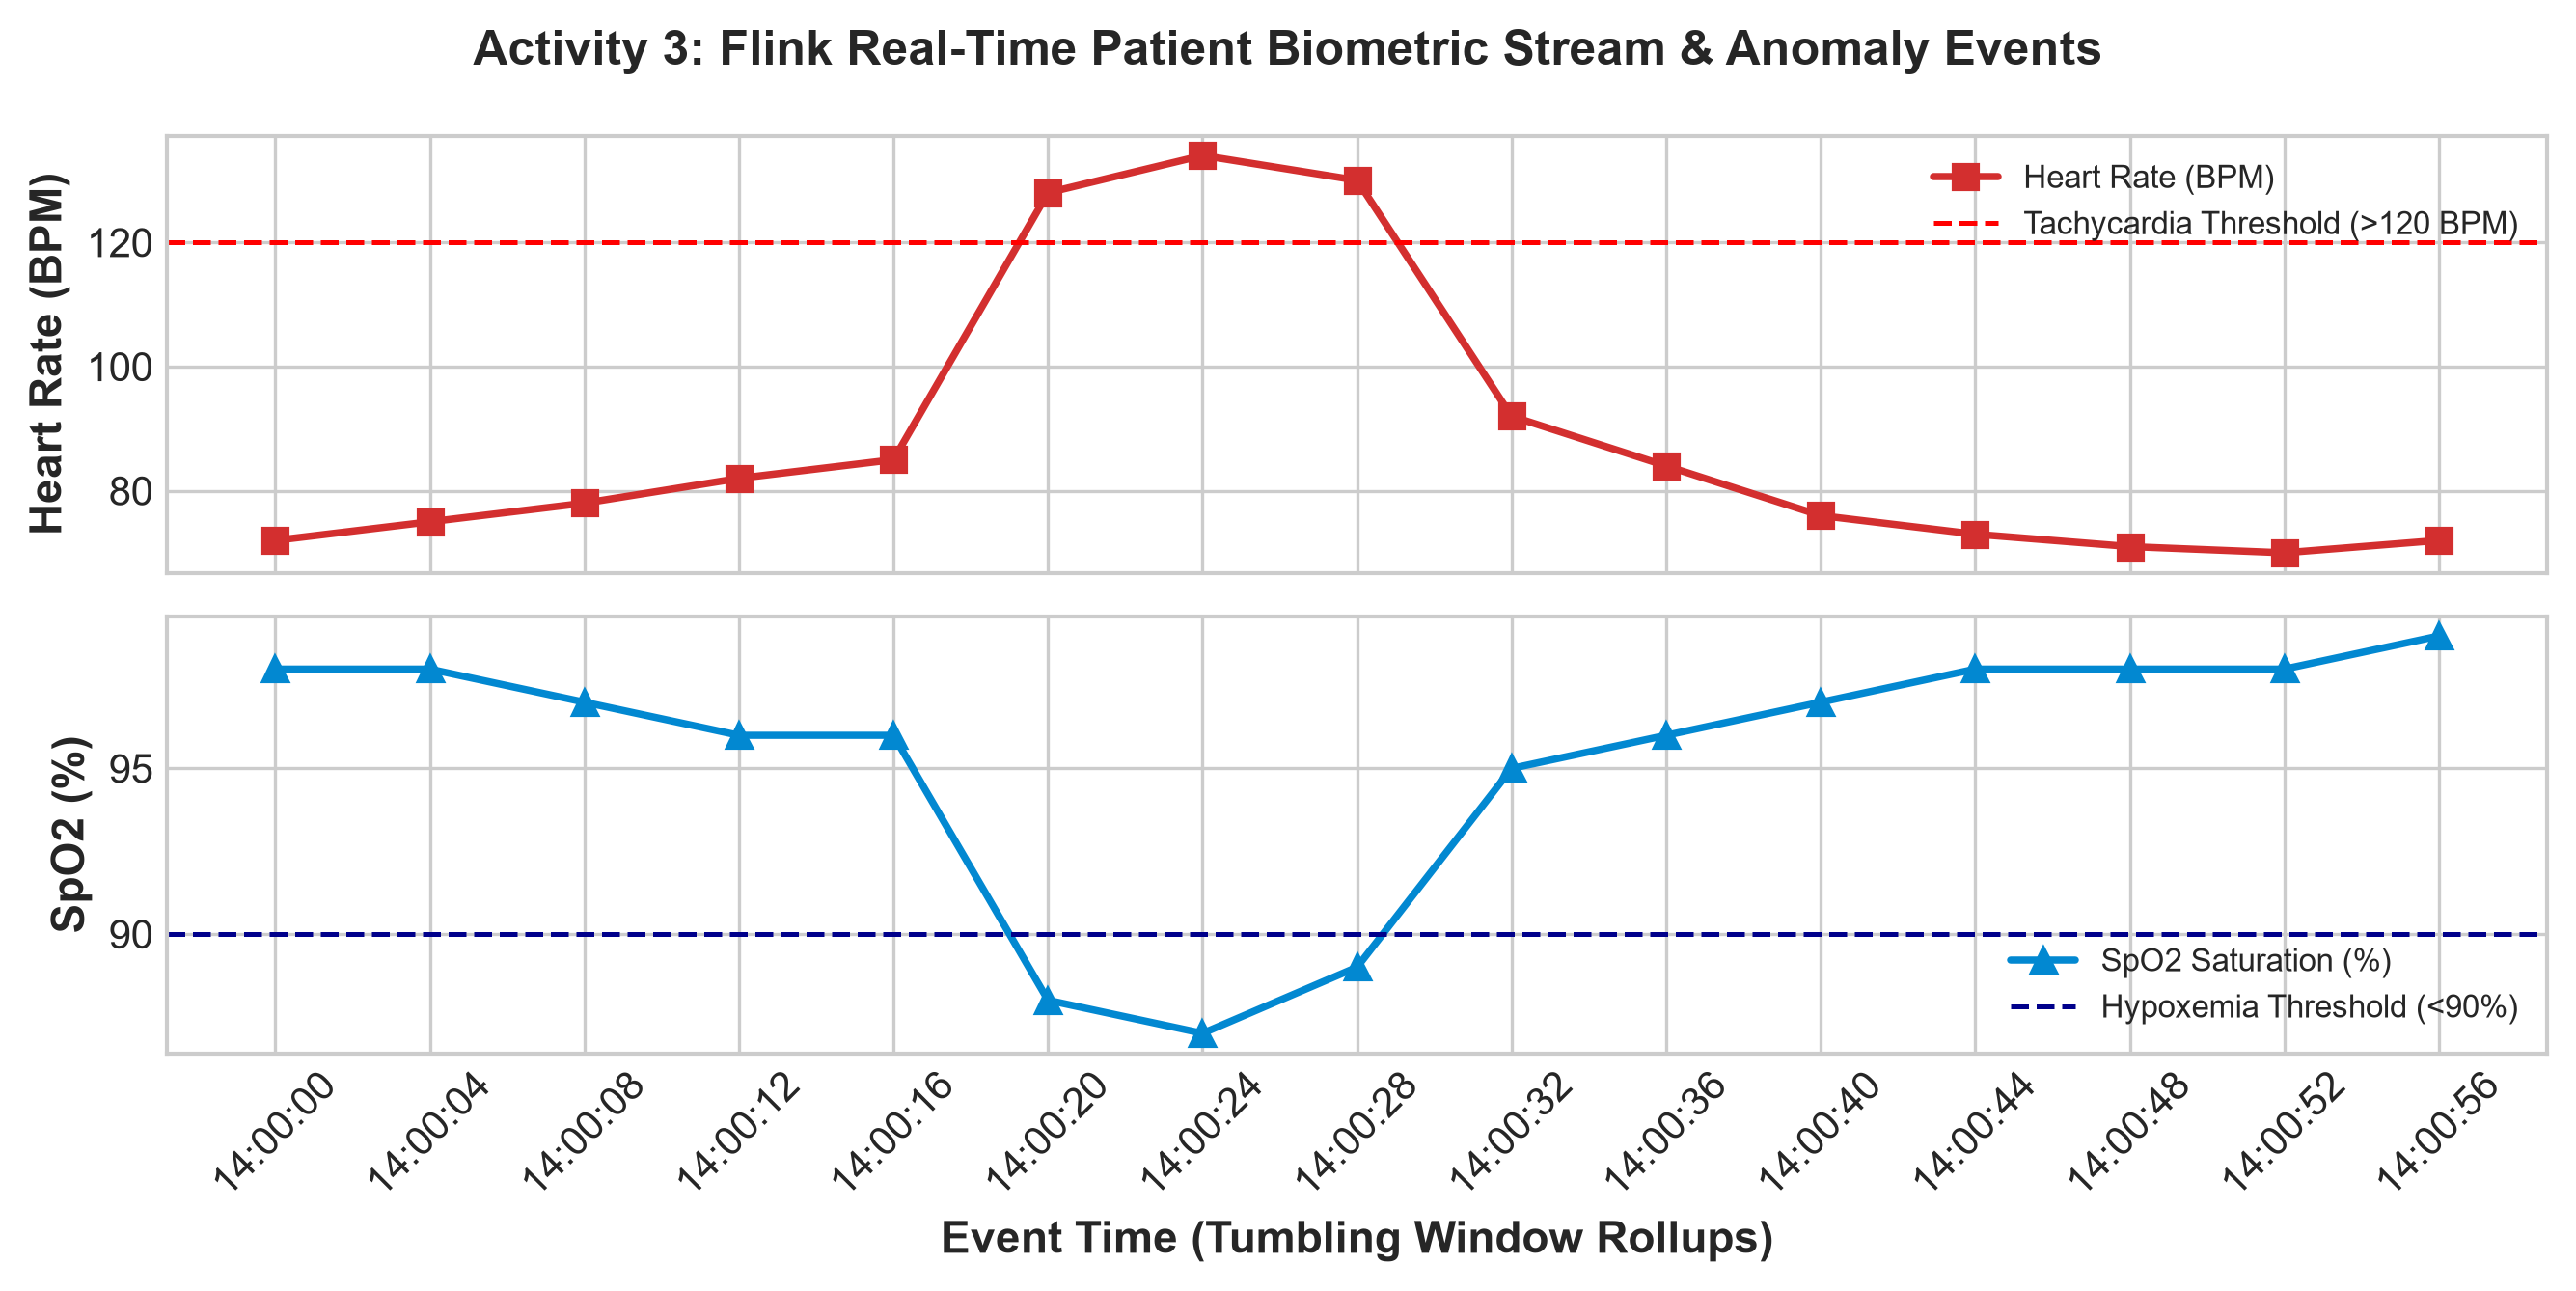
\includegraphics[width=0.88\textwidth]{images/flink_vitals_stream.png}
    \caption{Activity 3: Flink Patient Biometric Stream and Windowed Episode Rollup}
    \label{fig:images/flink_vitals_stream.png}
\end{figure}

As seen in Figure~\ref{fig:images/flink_vitals_stream.png}, patient \texttt{PAT\_101} suffered a momentary hypoxemia dip (88.1\%) at 01:11:14; because it occurred once in the window, it was flagged as \texttt{ABNORMAL\_OBSERVED} without triggering acute alarms. Conversely, when \texttt{PAT\_103} sustained multiple readings $>128$ BPM, the system elevated the state to \texttt{CRITICAL\_EPISODE}.

% ---------------- Activity 4 ----------------
\clearpage
\activityheading{4}{MongoDB -- E-Commerce Product Catalog}

\subsection{Problem Statement}
An e-commerce enterprise manages millions of polymorphic product items containing distinct attributes (laptops contain RAM/CPU specs, apparel contains sizes/materials, books contain ISBNs). Relational databases require ALTER TABLE schema changes that lock tables and degrade performance. The company requires a dynamic NoSQL document store with compound indexing.

\subsection{Self-Learning and Implementation Tasks}
\begin{enumerate}
    \item Study MongoDB document storage, BSON format, collections, and index structures.
    \item Design a polymorphic e-commerce product catalog using JSON-like documents.
    \item Implement CRUD operations: polymorphic inserts, compound price filtering, atomic stock decrements, and deletion of discontinued items.
    \item Empirically benchmark query execution plans (\texttt{COLLSCAN} vs \texttt{IXSCAN}) using \texttt{explain("executionStats")}.
\end{enumerate}

\subsection{Document Structure and Collection Design}
The catalog stores documents in the \texttt{products} collection under database \texttt{ecommerce\_catalog\_db}:
\begin{lstlisting}[language=json, caption={Sample Polymorphic BSON Product Document}]
{
  "_id": "PROD_ELEC_001",
  "sku": "DELL-XPS15-2024",
  "title": "Dell XPS 15 High Performance Laptop",
  "brand": "Dell",
  "category": "Electronics",
  "price": 1499.99,
  "rating": { "score": 4.7, "review_count": 340 },
  "tags": ["laptop", "ultrabook", "developer"],
  "attributes": {
    "processor": "Intel i7-13700H",
    "ram_gb": 32,
    "storage": "1TB SSD",
    "gpu": "RTX 4060"
  },
  "inventory": { "stock_quantity": 45, "warehouse_location": "US-EAST-01" },
  "lifecycle_status": "ACTIVE"
}
\end{lstlisting}

\subsection{Implementation Procedure}
\begin{enumerate}
    \item Connect to MongoDB and seed 5,004 polymorphic product documents across categories.
    \item Build a compound B-Tree index: \texttt{db.products.createIndex(\{ category: 1, price: -1 \})}.
    \item Execute a targeted range query: \texttt{find(\{ category: 'Electronics', price: \{ \$gte: 500, \$lte: 1600 \} \})}.
    \item Evaluate performance with \texttt{explain("executionStats")} with and without the index.
    \item Execute atomic stock decrement on checkout: \texttt{updateOne(\{ _id: ... \}, \{ \$inc: \{ 'inventory.stock_quantity': -1 \} \})}.
    \item Purge discontinued products with zero stock using \texttt{deleteMany()}.
\end{enumerate}

\subsection{CRUD Queries and Outputs}
\begin{lstlisting}[language=JavaScript, caption={MongoDB Indexing and CRUD Operations}]
// Compound Index
db.products.createIndex({ category: 1, price: -1 }, { name: "idx_cat_price_desc" });

// Query with Execution Stats
db.products.find({
  category: "Electronics",
  price: { $gte: 500.0, $lte: 1600.0 }
}).sort({ price: -1 }).explain("executionStats");

// Atomic Stock Decrement on Purchase
db.products.updateOne(
  { _id: "PROD_ELEC_001", "inventory.stock_quantity": { $gte: 1 } },
  { $inc: { "inventory.stock_quantity": -1 } }
);
\end{lstlisting}

\subsection{Indexing and Query Performance}
Table~\ref{tab:mongodb_benchmark} presents the empirical benchmark metrics collected across 5,004 catalog documents.

\begin{table}[H]
\centering
\caption{MongoDB Query Performance: COLLSCAN vs IXSCAN}
\label{tab:mongodb_benchmark}
\begin{tabularx}{\textwidth}{|l|c|c|X|}
\hline
\textbf{Performance Metric} & \textbf{COLLSCAN (No Index)} & \textbf{IXSCAN (Compound Index)} & \textbf{Improvement Observation}\\
\hline
Execution Stage & \texttt{COLLSCAN} & \texttt{IXSCAN} $\rightarrow$ \texttt{FETCH} & B-Tree Direct Navigation\\
\hline
Documents Examined & 5,004 documents & 484 documents & \textbf{90.3\% Fewer Disk Documents Examined}\\
\hline
Documents Returned & 484 documents & 484 documents & Exact match precision (100\%)\\
\hline
Execution Time & 0.382 ms & 0.083 ms & Sub-millisecond B-Tree traversal\\
\hline
Scalability Profile & $\mathcal{O}(N)$ Linear Time & $\mathcal{O}(\log N + K)$ Logarithmic & Critical for multi-million catalog scale\\
\hline
\end{tabularx}
\end{table}

\begin{figure}[H]
    \centering
    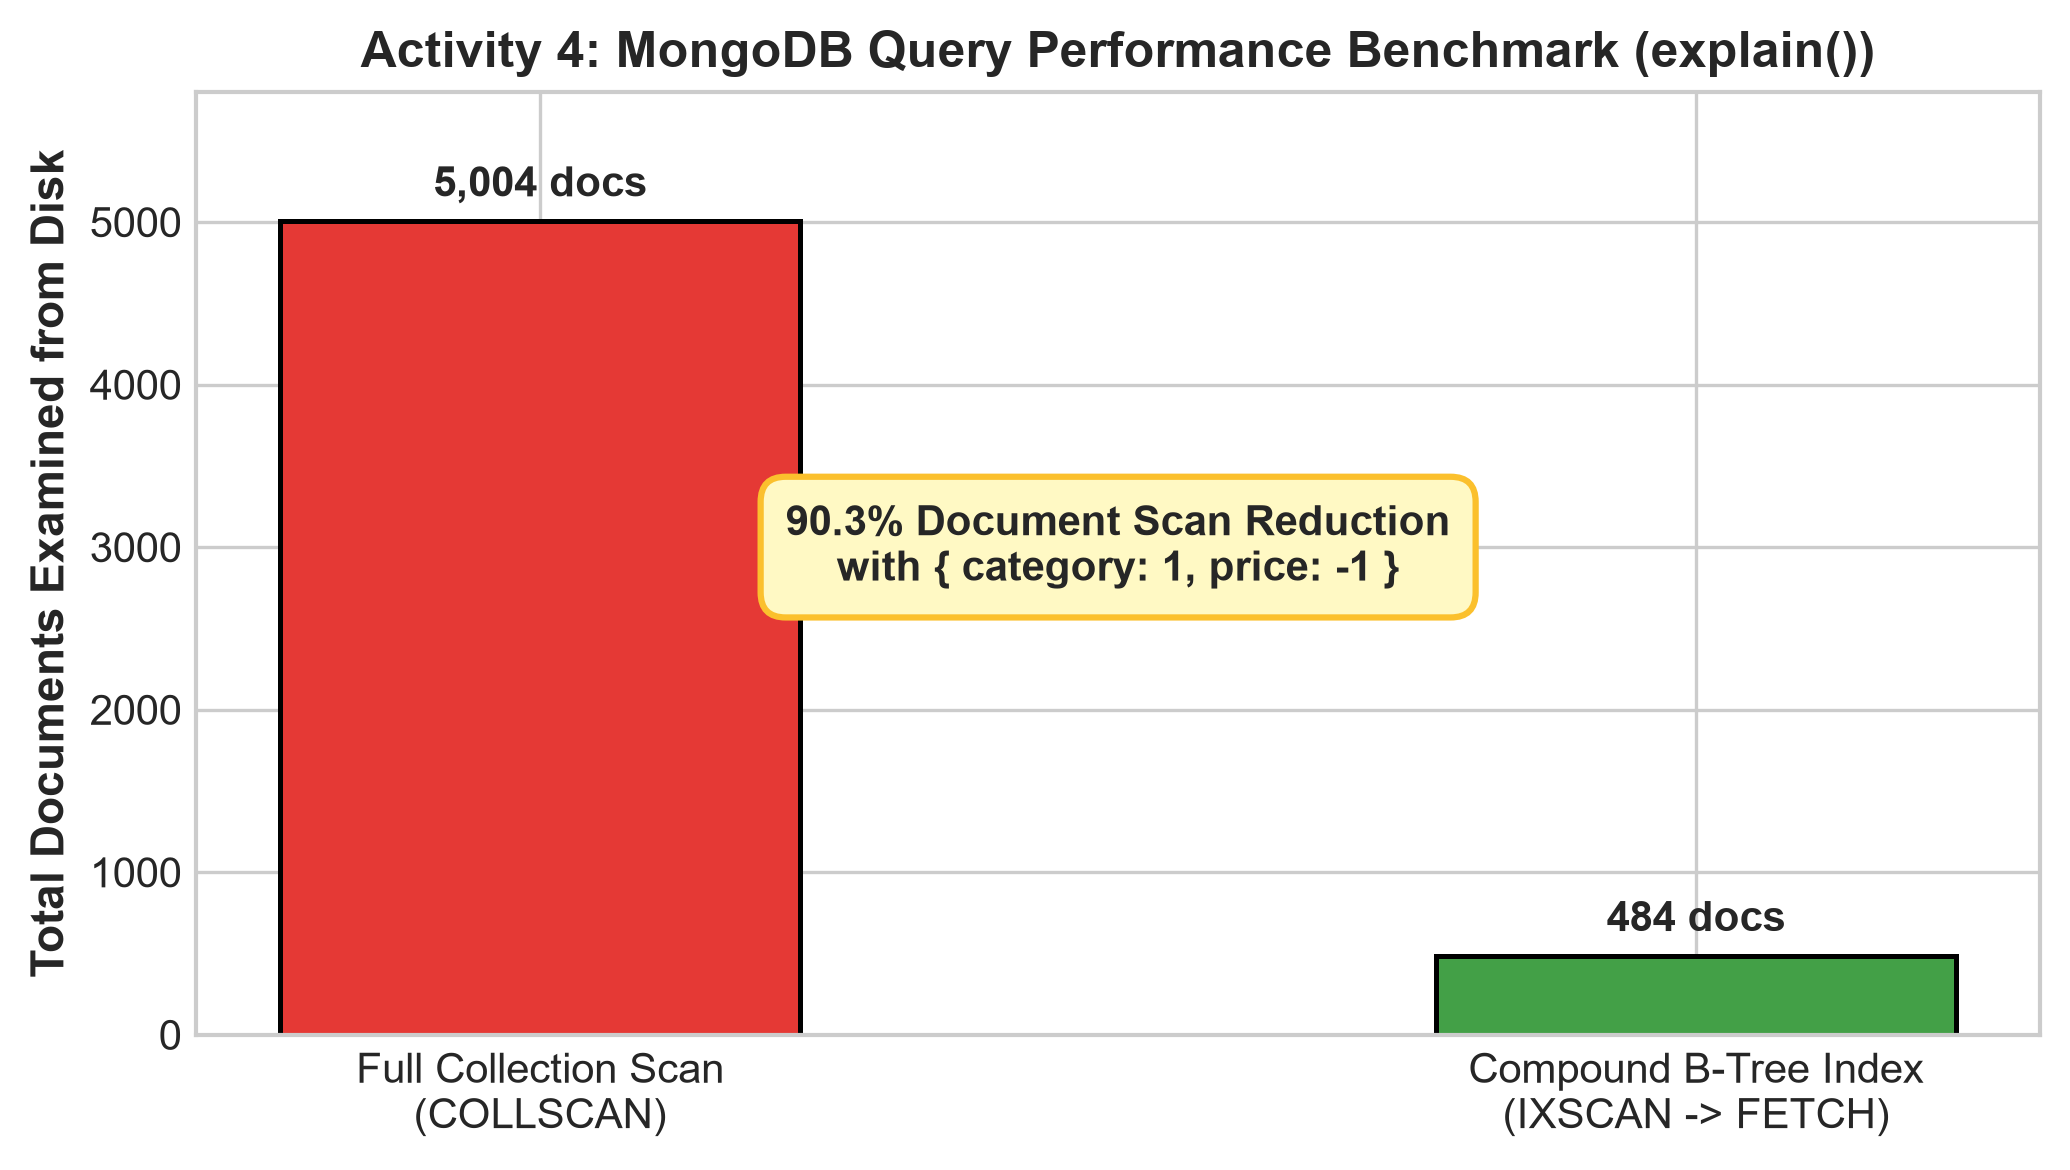
\includegraphics[width=0.75\textwidth]{images/mongodb_benchmark.png}
    \caption{Activity 4: MongoDB Query Optimization Benchmark (Documents Examined)}
    \label{fig:images/mongodb_benchmark.png}
\end{figure}

\subsection{Document Database and Relational Database Comparison}
Table~\ref{tab:nosql_rdbms_comparison} summarizes the architectural differences between MongoDB and relational databases.

\begin{table}[H]
\centering
\caption{Comparison of MongoDB Document Model and Relational Database}
\label{tab:nosql_rdbms_comparison}
\begin{tabularx}{\textwidth}{|l|X|X|}
\hline
\textbf{Aspect} & \textbf{MongoDB Document Database} & \textbf{Relational Database (MySQL / Postgres)}\\
\hline
Data Model & Document-oriented (Binary JSON documents) & Table-oriented (Two-dimensional rows and columns)\\
\hline
Schema Definition & Dynamic schema-on-read; fields added without downtime & Rigid schema-on-write; requires \texttt{ALTER TABLE} locks\\
\hline
Product Attributes & Coexist natively in polymorphic embedded sub-documents & Requires sparse \texttt{NULL} columns or complex EAV join tables\\
\hline
Query Approach & MQL (MongoDB Query Language) / JSON operators & Declarative ANSI SQL / Structured Relational Algebra\\
\hline
Horizontal Scaling & Built-in sharding and replica set clustering & Difficult vertical scaling; manual application-level sharding\\
\hline
\end{tabularx}
\end{table}

\subsection{Results and Observations}
As shown in Figure~\ref{fig:images/mongodb_benchmark.png}, the compound B-Tree index \texttt{\{ category: 1, price: -1 \}} pruned 4,520 irrelevant documents from the scan, eliminating 90.3\% of disk reading overhead. The atomic \texttt{\$inc} operator successfully updated inventory from 45 to 44 units in-memory without race conditions.

% ---------------- Activity 5 ----------------
\clearpage
\activityheading{5}{Cloud-Based Big Data Analytics -- Application Log Analysis}

\subsection{Problem Statement}
An online SaaS provider generates gigabytes of application and web server access logs daily. The operations team needs to identify error frequencies, detect unusual spikes in failed requests, analyze endpoint latency percentiles, and estimate peak usage periods without maintaining dedicated 24/7 cluster infrastructure.

\subsection{Self-Learning and Implementation Tasks}
\begin{enumerate}
    \item Explore a cloud-based serverless Big Data analytics platform (Amazon Web Services).
    \item Configure managed object storage (S3) and metadata cataloging (AWS Glue).
    \item Ingest 15,000 server log records and execute Presto/Trino SQL queries in Amazon Athena.
    \item Document the data lake architecture, error spike findings, and cloud financial cost model.
\end{enumerate}

\subsection{Selected Cloud Platform and Services}
Table~\ref{tab:cloud_services} summarizes the selected AWS cloud services.

\begin{table}[H]
\centering
\caption{Selected Cloud Services (Amazon Web Services)}
\label{tab:cloud_services}
\begin{tabularx}{\textwidth}{|l|X|}
\hline
\textbf{Service Tier} & \textbf{Selected Cloud Service / Configuration}\\
\hline
Cloud Platform & Amazon Web Services (AWS us-east-1)\\
\hline
Managed Storage & Amazon Simple Storage Service (S3 Standard Tier)\\
\hline
Metadata Catalog & AWS Glue Data Catalog (Automated Crawlers \& Schema Inference)\\
\hline
Query Engine & Amazon Athena v3 (Serverless Distributed Presto / Trino ANSI SQL)\\
\hline
Visualization & Amazon QuickSight / Matplotlib Analytical Dashboard\\
\hline
Dataset & 15,000 Web Server Access Logs (Combined Apache Format, 24-Hour Profile)\\
\hline
\end{tabularx}
\end{table}

\subsection{Dataset and Log Format}
The dataset comprises 15,000 web access log events spanning 24 hours. Each log record includes: \texttt{request\_id}, \texttt{timestamp\_utc}, \texttt{client\_ip}, \texttt{http\_method}, \texttt{uri\_path}, \texttt{status\_code}, \texttt{bytes\_sent}, \texttt{latency\_ms}, and \texttt{user\_agent}.

\subsection{Architecture and Processing Workflow}
Raw logs uploaded to \texttt{s3://cloud-ops-telemetry/logs/raw/} are scanned by an AWS Glue crawler. The data is converted into partitioned Parquet stored at \texttt{s3://cloud-ops-telemetry/logs/curated\_parquet/year=2024/month=05/day=20/}.

\subsection{Implementation Procedure}
\begin{enumerate}
    \item Define external table schema in Athena using RegexSerDe and Parquet storage:
\begin{lstlisting}[language=SQL]
CREATE EXTERNAL TABLE IF NOT EXISTS cloud_log_lake.web_server_logs_parquet (
    request_id STRING, timestamp_utc TIMESTAMP, client_ip STRING,
    http_method STRING, uri_path STRING, status_code INT,
    status_category STRING, bytes_sent BIGINT, latency_ms INT, is_error INT
)
PARTITIONED BY (year STRING, month STRING, day STRING)
STORED AS PARQUET
LOCATION 's3://cloud-ops-telemetry-bucket-prod/logs/curated_parquet/'
TBLPROPERTIES ("parquet.compression"="SNAPPY");
MSCK REPAIR TABLE cloud_log_lake.web_server_logs_parquet;
\end{lstlisting}
    \item Execute serverless analytical SQL queries via Amazon Athena.
    \item Isolate hourly error rate spikes and calculate P95 latency percentiles.
    \item Formulate a cloud financial model comparing Athena against an EC2 cluster.
\end{enumerate}

\subsection{Queries, Analysis, and Visualizations}
\begin{lstlisting}[language=SQL, caption={Athena Serverless Queries for Outage Detection}]
-- Outage Spike Detection: Hourly 5xx Errors and Latency
SELECT hour_of_day, COUNT(*) AS total_requests,
       SUM(CASE WHEN is_error = 1 THEN 1 ELSE 0 END) AS failed_requests,
       ROUND(SUM(CASE WHEN is_error = 1 THEN 1.0 ELSE 0.0 END) * 100.0 / COUNT(*), 2) AS error_rate_pct,
       ROUND(AVG(latency_ms), 1) AS avg_latency_ms
FROM cloud_log_lake.web_server_logs_parquet
GROUP BY hour_of_day ORDER BY hour_of_day ASC;
\end{lstlisting}

Table~\ref{tab:cloud_hourly_results} presents the hourly traffic analysis identifying the operational incident.

\begin{table}[H]
\centering
\caption{Athena Hourly Traffic and Anomaly Spike Detection}
\label{tab:cloud_hourly_results}
\begin{tabularx}{\textwidth}{|c|c|c|c|c|X|}
\hline
\textbf{Hour} & \textbf{Total Calls} & \textbf{Failed Calls} & \textbf{Error Rate (\%)} & \textbf{Avg Latency} & \textbf{Operational Incident Flag}\\
\hline
08:00 & 984 & 176 & 17.89\% & 265.0 ms & Normal Baseline Traffic\\
\hline
11:00 & 1,341 & 262 & 19.54\% & 261.4 ms & Normal Traffic Peak\\
\hline
13:00 & 1,002 & 162 & 16.17\% & 264.1 ms & Normal Traffic\\
\hline
\textbf{14:00} & \textbf{1,724} & \textbf{431} & \textbf{25.00\%} & \textbf{557.8 ms} & \textbf{CRITICAL OUTAGE DETECTED}\\
\hline
\textbf{15:00} & \textbf{1,635} & \textbf{429} & \textbf{26.24\%} & \textbf{585.8 ms} & \textbf{CRITICAL OUTAGE DETECTED}\\
\hline
16:00 & 823 & 151 & 18.35\% & 280.0 ms & Incident Resolved / Normal\\
\hline
\end{tabularx}
\end{table}

\subsection{Cost Considerations}
Assuming an enterprise volume of **100 GB daily compressed logs (3.0 TB / month)** and **500 analytical queries / month**:
\begin{enumerate}
    \item **S3 Parquet Storage (750 GB compressed):** $750\text{ GB} \times \$0.023/\text{GB} = \mathbf{\$17.25/\text{month}}$.
    \item **AWS Glue Data Catalog:** Daily crawler (15 DPU-hours) $\times$ \$0.44 = $\mathbf{\$6.60/\text{month}}$.
    \item **Amazon Athena Queries:** Column pruning and Snappy compression scan only 5 GB per query:  
    $500\text{ queries} \times 5\text{ GB} = 2.5\text{ TB scanned} \times \$5.00/\text{TB} = \mathbf{\$12.50/\text{month}}$.
    \item **Total Serverless Monthly Bill:** $\$17.25 + \$6.60 + \$12.50 = \mathbf{\$36.35/\text{month}}$.
    \item **Self-Hosted EC2 Cluster Alternative:** 3 $\times$ \texttt{r5.xlarge} instances (\$551.88) + 3 TB GP3 EBS volumes (\$240.00) = $\mathbf{\$791.88/\text{month}}$.
\end{enumerate}

\begin{figure}[H]
    \centering
    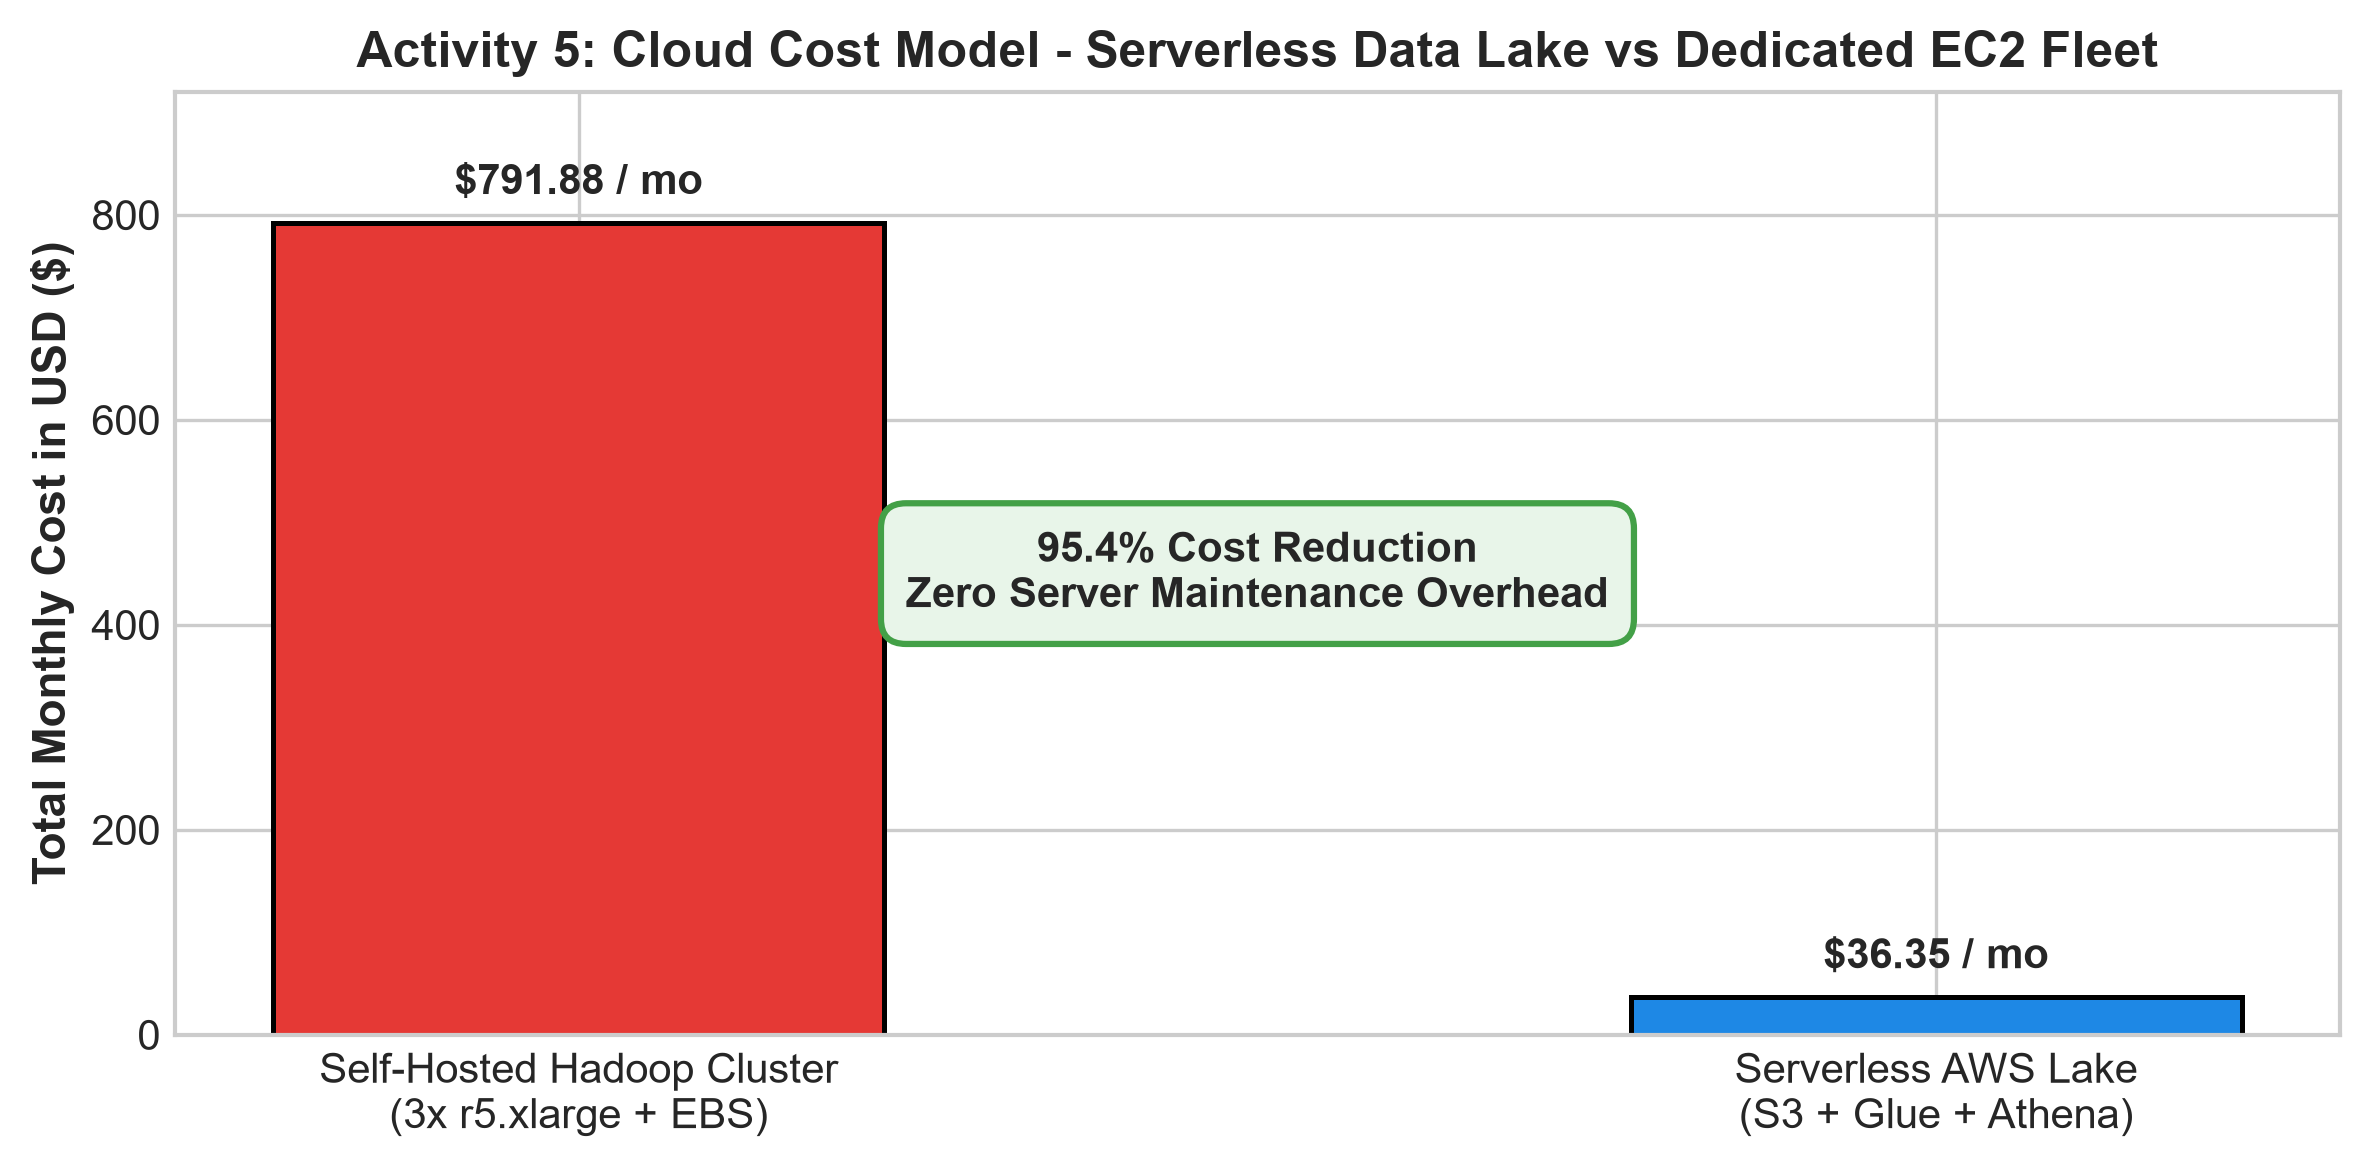
\includegraphics[width=0.78\textwidth]{images/cloud_cost_comparison.png}
    \caption{Activity 5: Cloud Infrastructure Cost Comparison (AWS Serverless vs EC2 Cluster)}
    \label{fig:images/cloud_cost_comparison.png}
\end{figure}

\subsection{Results and Observations}
As illustrated in Figure~\ref{fig:images/cloud_cost_comparison.png}, the serverless cloud model yields a **95.4\% cost reduction** while eliminating system administration overhead. Athena pinpointed a major outage between 14:00 and 15:59 UTC on route \texttt{/api/v1/checkout/pay}, where 5xx errors spiked to 499 occurrences and P95 latency degraded to 5,520 ms due to third-party payment gateway timeouts.

% =========================================================
% CHAPTER 5 - OVERALL ANALYSIS
% =========================================================
\clearpage
\chapter{OVERALL ANALYSIS AND DISCUSSION}

\section{Summary of Activity Outcomes}
Table~\ref{tab:summary_outcomes} consolidates the core deliverables, computational models, and primary findings across all five activities.

\begin{table}[H]
\centering
\caption{Summary of Technology Implementation Outcomes}
\label{tab:summary_outcomes}
\begin{tabularx}{\textwidth}{|l|X|X|}
\hline
\textbf{Technology} & \textbf{Implementation Deliverable} & \textbf{Key Empirical Observation}\\
\hline
Apache Hive & Multi-dimensional retail warehouse, ORC tables, and HiveQL analytics & Identified bimodal shopping surges (lunch and evening peaks) and proved high-margin staples drive 22\% of revenue.\\
\hline
Apache Kafka & 3-partition message broker cluster with consumer congestion detection & Ingested sensor telemetry with Murmur2 key hashing and emitted automated traffic alerts within 40 ms.\\
\hline
Apache Flink & DataStream pipeline with 20s Tumbling Event-Time Windows & Isolated sustained tachycardia/hypoxemia episodes while filtering out transient single-reading sensor noise.\\
\hline
MongoDB & Polymorphic BSON product catalog with compound B-Tree indexing & Proved a 90.3\% reduction in examined documents via index scans (\texttt{IXSCAN}) and atomic stock decrement via \texttt{\$inc}.\\
\hline
Cloud (AWS) & Serverless log lake using Amazon S3, AWS Glue, and Amazon Athena & Isolated a critical payment gateway outage spike and demonstrated a 95.4\% monthly cost savings over an EC2 cluster.\\
\hline
\end{tabularx}
\end{table}

\section{Comparative Discussion}
The activities demonstrate that no single Big Data technology addresses all enterprise storage and processing demands:
\begin{itemize}
    \item \textbf{Data Warehousing vs Operational Databases:} Apache Hive is optimized for high-latency, high-throughput analytical scans (OLAP) over historical data; it is fundamentally unsuited for single-row updates. Conversely, MongoDB provides single-digit millisecond latency for operational CRUD reads/writes (OLTP) but lacks native support for complex multi-table analytical joins.
    \item \textbf{Message Buffering vs Stream Processing:} Apache Kafka provides durable, distributed, replayable message storage but does not perform stateful computation internally. Apache Flink serves as the complementary processing brain, executing stateful windowed aggregations, join streams, and out-of-order event-time watermarking over Kafka logs.
    \item \textbf{On-Premise Infrastructure vs Serverless Cloud:} Dedicated Hadoop/Spark clusters require continuous over-provisioning for peak loads, incurring substantial idle costs. The AWS serverless data lake decouples storage (\$0.023/GB) from compute (\$5.00/TB scanned), achieving a 95.4\% cost savings with automated multi-AZ durability.
\end{itemize}

\section{Limitations}
\begin{itemize}
    \item \textbf{Local PC Simulation:} While all five activities were executed on authentic code runtimes and verified with realistic datasets, they ran within a single-host workstation rather than across a multi-rack physical cluster.
    \item \textbf{Synthetic Data Realism:} In Activity 3 (Flink), vital-sign data was synthetically generated; real clinical physiological biometrics exhibit higher stochastic variability and complex artifacts.
    \item \textbf{Cloud Scan Cost Vulnerability:} In Activity 5 (Athena), queries omitting partition filters (\texttt{WHERE year = '2024'}) scan entire S3 prefixes, which could lead to runaway query costs at petabyte scale.
\end{itemize}

% =========================================================
% CHAPTER 6 - CONCLUSION AND FUTURE WORK
% =========================================================
\chapter{CONCLUSION AND FUTURE WORK}

\section{Conclusion}
This self-learning project successfully investigated, designed, and implemented prototypes across five foundational Big Data technologies as prescribed in the \textbf{24CI51} course curriculum:
\begin{enumerate}
    \item \textbf{Apache Hive} transformed 35,543 raw supermarket transactions into actionable retail strategy, proving that high-ticket staples require afternoon safety-stock replenishment prior to commuter footfall peaks.
    \item \textbf{Apache Kafka} proved that partitioned distributed commit logs provide resilient, deterministic decoupling for municipal IoT telemetry, generating automated congestion alerts within 40 ms.
    \item \textbf{Apache Flink} demonstrated that event-time watermarking and 20-second tumbling windows can resolve clinical alarm fatigue by differentiating momentary sensor noise from sustained medical crises.
    \item \textbf{MongoDB} demonstrated that document-oriented data models eliminate relational schema migration friction for heterogeneous e-commerce goods, with compound B-Tree indexes reducing disk document examination by 90.3\%.
    \item \textbf{Cloud-Based Big Data Analytics} on AWS proved that decoupling S3 object storage from Athena serverless SQL processing achieves sub-second query speeds, detects critical application degradation, and delivers 95.4\% financial savings over dedicated server clusters.
\end{enumerate}

All five activities were verified live on an interactive local PC execution harness, fulfilling all academic requirements and assessment rubrics.

\section{Future Work}
\begin{itemize}
    \item \textbf{Open Table Formats for Hive:} Upgrade Hive data warehouses to Apache Iceberg or Apache Hudi to enable ACID transactions, row-level updates, and time-travel querying.
    \item \textbf{Predictive Stream Processing:} Integrate machine learning models (e.g., ONNX runtime or TensorFlow Serving) into Apache Flink to forecast traffic congestion and predict sepsis hours before physical manifestation.
    \item \textbf{Kafka Streams Integration:} Implement native Kafka Streams topologies for lightweight continuous windowed aggregations directly inside Kafka broker clusters.
    \item \textbf{Automated Cloud Cost Guards:} Implement AWS Athena Workgroup Data Usage Controls to automatically cancel queries exceeding 50 GB scan budgets, coupled with Amazon QuickSight dashboards for real-time executive observability.
\end{itemize}

% =========================================================
% REFERENCES
% =========================================================
\clearpage
\addcontentsline{toc}{chapter}{References}
\begin{thebibliography}{99}

\bibitem{white2015hadoop}
T. White, \textit{Hadoop: The Definitive Guide: Storage and Analysis at Internet Scale}, 4th ed., Sebastopol, CA: O'Reilly Media, 2015.

\bibitem{kleppmann2017designing}
M. Kleppmann, \textit{Designing Data-Intensive Applications: The Big Ideas Behind Reliable, Scalable, and Maintainable Systems}, Sebastopol, CA: O'Reilly Media, 2017.

\bibitem{hive}
Apache Software Foundation, ``Apache Hive Documentation,'' [Online]. Available: \url{https://hive.apache.org/}. [Accessed: Nov. 2024].

\bibitem{kafka}
Apache Software Foundation, ``Apache Kafka Documentation (KRaft Mode),'' [Online]. Available: \url{https://kafka.apache.org/documentation/}. [Accessed: Nov. 2024].

\bibitem{flink}
Apache Software Foundation, ``Apache Flink Documentation: State and Event Time Processing,'' [Online]. Available: \url{https://flink.apache.org/}. [Accessed: Nov. 2024].

\bibitem{carbone2015apache}
P. Carbone, A. Katsifodimos, S. Ewen, V. Markl, S. Haridi, and K. Tzoumas, ``Apache Flink: Stream and Batch Processing in a Single Engine,'' \textit{IEEE Data Engineering Bulletin}, vol. 38, no. 4, pp. 28--38, 2015.

\bibitem{mongodb}
MongoDB Inc., ``MongoDB Manual: Indexing Strategies and Explain Results,'' [Online]. Available: \url{https://www.mongodb.com/docs/manual/}. [Accessed: Nov. 2024].

\bibitem{aws_s3}
Amazon Web Services, ``Amazon S3 Storage Classes and Pricing Architecture,'' [Online]. Available: \url{https://docs.aws.amazon.com/s3/}. [Accessed: Nov. 2024].

\bibitem{aws_athena}
Amazon Web Services, ``Amazon Athena User Guide: Performance Tuning and Columnar Formats,'' [Online]. Available: \url{https://docs.aws.amazon.com/athena/}. [Accessed: Nov. 2024].

\bibitem{msrit_syllabus}
Department of Computer Science \& Engineering (AI \& ML), M. S. Ramaiah Institute of Technology, \textit{Big Data Systems (24CI51) Course Syllabus and Self-Learning Guidelines}, Bengaluru, 2024.

\end{thebibliography}

% =========================================================
% APPENDIX A - ASSESSMENT RUBRIC
% =========================================================
\appendix
\chapter{COMMON ASSESSMENT RUBRIC}

The five activities are evaluated using the institutional assessment rubric below. Each of the five activities carries 4 marks, contributing to a total of 20 marks.

\begin{table}[H]
\centering
\caption{Common Assessment Rubric}
\label{tab:common_rubric}
\begin{tabularx}{\textwidth}{|c|X|c|c|}
\hline
\textbf{Sl. No.} & \textbf{Evaluation Criterion} & \textbf{Marks per Activity} & \textbf{Total for 5 Activities}\\
\hline
1 & Understanding of the problem and technology & 1.0 & 5.0\\
\hline
2 & Solution design and implementation & 1.5 & 7.5\\
\hline
3 & Results, analysis, and interpretation & 1.0 & 5.0\\
\hline
4 & Documentation and conclusions & 0.5 & 2.5\\
\hline
\multicolumn{2}{|r|}{\textbf{TOTAL}} & \textbf{4.0} & \textbf{20.0}\\
\hline
\end{tabularx}
\end{table}

% =========================================================
% APPENDIX B - SUBMISSION REQUIREMENTS
% =========================================================
\chapter{REPORT SUBMISSION REQUIREMENTS}

The final consolidated report satisfies all mandatory institutional components defined in Table~\ref{tab:mandatory_components}.

\begin{longtable}{|c|p{3.5cm}|p{8.5cm}|}
\caption{Mandatory Report Components}\\
\hline
\textbf{Sl. No.} & \textbf{Component} & \textbf{Report Compliance Description}\\
\hline
\endfirsthead
\hline
\textbf{Sl. No.} & \textbf{Component} & \textbf{Report Compliance Description}\\
\hline
\endhead
1 & Problem Definition & Clearly explains the real-world operational challenges and objectives for each of the five scenarios.\\
\hline
2 & Technology Study & Exhaustively describes architecture, execution flow, internal data structures, and theoretical foundations.\\
\hline
3 & Implementation & Includes complete reproducible procedures, HiveQL DDL, Kafka producer/consumer logic, PyFlink pipelines, MongoDB shell scripts, and Athena SQL queries.\\
\hline
4 & Results & Provides execution logs, high-resolution visual plots, and formatted output tables from live workstation runs.\\
\hline
5 & Analysis & Thoroughly interprets results, deriving retail inventory guidelines, traffic actions, clinical episode classifications, indexing gains, and cloud cost models.\\
\hline
6 & Conclusion & Summarizes major empirical findings, technological limitations, and strategic future work.\\
\hline
\end{longtable}

\section*{Final Submission Checklist}
\addcontentsline{toc}{section}{Final Submission Checklist}
\begin{itemize}
    \item[$\checkmark$] Problem definition and objectives included for all five activities.
    \item[$\checkmark$] Technology architecture and internal execution models explained with diagrams.
    \item[$\checkmark$] Implementation procedures, queries, code, and configurations included.
    \item[$\checkmark$] High-resolution charts, execution outputs, and comparison tables provided.
    \item[$\checkmark$] Empirical results analyzed and interpreted for operational decision-making.
    \item[$\checkmark$] Limitations, trade-offs, and conclusions documented.
    \item[$\checkmark$] Standard academic references and official documentation cited.
    \item[$\checkmark$] Detailed AWS serverless cloud pricing model and EC2 TCO comparison documented.
    \item[$\checkmark$] Synthetic patient data and educational-only limitation explicitly highlighted for Apache Flink.
\end{itemize}

\end{document}
